\ifdefined\PRESENTATION\else\PassOptionsToClass{handout}{beamer}\fi\documentclass[aspectratio=169, lualatex]{beamer}
\makeatletter\def\input@path{{theme/}}\makeatother\usetheme{cipher}

\title{Applied Cryptography - 2.4: End-to-End Encrypted Cloud Storage}
\author{Nadim Kobeissi}
\subject{An exploration of end-to-end encrypted cloud storage systems, their security challenges, and cryptographic attacks on real-world implementations.}
\keywords{end-to-end encryption, cloud storage, MEGA, Nextcloud, cryptographic attacks, key management, authentication, OPAQUE, SRP, password security, WhatsApp, passkeys}
\institute{Symbolic Software}
\instituteimage{images/symbolicsoft-white.png}
\date{\today}
\coversubtitle{Summer 2026}
\coverpartname{Part 2: Real-World Cryptography}
\covertopicname{2.4: End-to-End Encrypted Cloud Storage}
\coverwebsite{https://appliedcryptography.page}

\begin{document}
\begin{frame}[plain]
	\titlepage
\end{frame}

\section{Introduction}

\begin{frame}{Cloud storage today}
	\begin{columns}[c]
		\begin{column}{0.5\textwidth}
			\begin{itemize}
				\item Cloud storage is a prevalent computing paradigm today
				\item Outsources data storage to third-party services
				\item Benefits for users:
				      \begin{itemize}
					      \item No need to worry about backups
					      \item High data availability
					      \item Access data from anywhere
				      \end{itemize}
				\item The major providers (Google, Microsoft, Amazon, and Apple by default) hold the encryption keys
			\end{itemize}
		\end{column}
		\begin{column}{0.5\textwidth}
			\imagewithcaption{onedrive.png}{Microsoft OneDrive is an example of a popular cloud storage service.}
		\end{column}
	\end{columns}
\end{frame}

\begin{frame}{Regular vs end-to-end encrypted cloud storage}
	\begin{columns}
		\begin{column}{0.5\textwidth}
			\textbf{Regular Cloud Storage}\\
			\textit{(e.g., OneDrive, Google Drive)}
			\vspace{0.5cm}
			\begin{itemize}[<+->]
				\item \textbf{Transport encryption:} TLS protects data in transit
				\item \textbf{Encryption at rest:} Provider encrypts on their servers
				\item \textbf{Provider controls keys:} Can decrypt your data
			\end{itemize}
		\end{column}
		\begin{column}{0.5\textwidth}
			\textbf{E2E Encrypted Storage}\\
			\textit{(e.g., MEGA, Nextcloud)}
			\vspace{0.5cm}
			\begin{itemize}[<+->]
				\item \textbf{Client-side encryption:} Data encrypted before upload
				\item \textbf{User controls keys:} Provider never sees plaintext
				\item \textbf{Confidentiality:} Provider learns nothing about content
			\end{itemize}
		\end{column}
	\end{columns}
\end{frame}

\begin{frame}{Regular vs end-to-end encrypted cloud storage}
	\begin{columns}
		\begin{column}{0.5\textwidth}
			\textbf{Regular Cloud Storage}\\
			\textit{(e.g., OneDrive, Google Drive)}
			\\
			\vspace{0.5cm}
			\textbf{Risks:}
			\begin{itemize}[<+->]
				\item Provider breach exposes data
				\item Government requests
				\item Insider threats
				\item Provider can analyze content
			\end{itemize}
		\end{column}
		\begin{column}{0.5\textwidth}
			\textbf{E2E Encrypted Storage}\\
			\textit{(e.g., MEGA, Nextcloud)}
			\\
			\vspace{0.5cm}
			\textbf{Guarantees:}
			\begin{itemize}[<+->]
				\item Provider breach reveals only ciphertext
				\item Government gets encrypted data
				\item No insider access to content
				\item Provider can only analyze metadata
			\end{itemize}
		\end{column}
	\end{columns}
\end{frame}

\begin{frame}{The threat model: a malicious provider}
	\begin{itemize}
		\item The last two slides say what E2EE storage \textit{promises}. To check the promise, we have to say what the adversary can do
		\item \textbf{Honest-but-curious server:} follows the protocol, but reads everything it stores and sees
		\item \textbf{Malicious server:} may also \textit{modify} what it stores and \textit{lie} in protocol messages
		      \begin{itemize}
			      \item A breached provider, a rogue insider, or a provider under legal compulsion all look like this
		      \end{itemize}
		\item What E2EE storage should guarantee even against a malicious server:
		      \begin{itemize}
			      \item \textbf{Confidentiality:} file contents stay secret
			      \item \textbf{Integrity:} tampered or forged files are detected by the client
		      \end{itemize}
		\item Keep this in mind: every attack in this lecture is carried out \textit{by the server}
	\end{itemize}
\end{frame}

\begin{frame}{Key management challenges}
	\begin{itemize}
		\item E2EE hands key management to the user --- and humans cannot memorize 256-bit keys
		\item So in practice, everything is bootstrapped from a \textbf{password}
		\item Fundamental limitation: passwords come from a small space, so \textbf{dictionary attacks} are always on the table
		\item A slow key derivation function buys time; it does not change the size of the space
		\item Every design in this lecture is, at bottom, a different answer to the same question: how do we get from a password to a key without letting the server guess the password?
	\end{itemize}
\end{frame}

\begin{frame}{Password hashing}
	\begin{columns}[c]
		\begin{column}{1\textwidth}
			\begin{itemize}
				\item Users typically access E2EE storage via passwords
				\item Passwords must be converted to cryptographic keys
				\item Common approach: password hashing\footnote{This was previously covered in topic 1.6: \textit{Collision-Resistant Hash Functions}.}
				\item Popular password hashing functions:
				      \begin{itemize}
					      \item \textbf{PBKDF2}: Widely deployed but aging
					      \item \textbf{scrypt}: Memory-hard against ASICs
					      \item \textbf{Argon2}: Winner of Password Hashing Competition
				      \end{itemize}
				\item KDFs slow down brute-force attacks
				\item Still vulnerable to dictionary attacks with weak passwords
			\end{itemize}
		\end{column}
	\end{columns}
\end{frame}

\begin{frame}{The authentication vs encryption dilemma}
	\begin{itemize}
		\item Traditional services: the server stores a password hash and checks your password at login
		\item E2EE requirement: the server must never learn the key that encrypts your data
		\item So one password must do two jobs, and the server may only see one of them:
		      \begin{itemize}
			      \item \textbf{Two passwords:} one for login, one for encryption (Proton Mail offers this as an option) --- nobody wants two passwords
			      \item \textbf{One password, two derived keys:} stretch it, send half of the output to the server as an \textit{authentication key}, keep the other half as the \textit{encryption key} --- MEGA's approach
			      \item \textbf{Password-authenticated key exchange (PAKE):} prove you know the password without the server ever holding a password-equivalent --- SRP, OPAQUE; more later
			      \item \textbf{Hardware-backed:} passkeys, Secure Enclave --- requires specific devices or platforms
		      \end{itemize}
	\end{itemize}
\end{frame}

\begin{frame}{The mud puddle test}
	\begin{columns}[c]
		\begin{column}{1\textwidth}
			\begin{itemize}
				\item \textbf{What is the mud puddle test?}\footnote{Coined by cryptographer Matthew Green in 2012: \url{https://blog.cryptographyengineering.com/2012/04/05/icloud-who-holds-key/}}
				      \begin{itemize}
					      \item Thought experiment for E2EE systems
					      \item ``If you drop your device in a mud puddle and it's destroyed\ldots''
					      \item ``And then slip in that mud puddle and suffer from password amnesia\ldots''
					      \item ``\ldots can you recover your data on a new device?''
				      \end{itemize}
				\item \textbf{In true E2EE:}
				      \begin{itemize}
					      \item Lost password = lost data forever
					      \item No backdoor for the provider
					      \item No ``forgot password'' that maintains E2EE
				      \end{itemize}
				\item \textbf{The fundamental trade-off:}
				      \begin{itemize}
					      \item Security vs recoverability
					      \item Provider can't help without breaking E2EE
				      \end{itemize}
			\end{itemize}
		\end{column}
	\end{columns}
\end{frame}

\begin{frame}{Password recovery expectations vs reality}
	\begin{itemize}
		\item \textbf{What users expect} (trained by Gmail, Facebook, \ldots): ``forgot password'' always works, and data is never permanently lost
		\item \textbf{What E2EE providers can offer instead:}
		      \begin{itemize}
			      \item \textbf{Recovery keys:} a long random string the user must store somewhere safe --- routinely lost or never written down (Apple ADP and WhatsApp's 64-digit key, both coming up)
			      \item \textbf{Social recovery:} split the key among trusted contacts, any $t$ of $n$ can restore it --- setup is complex, and the contacts must be trusted
			      \item \textbf{Security questions:} familiar, but weak against anyone who knows you
		      \end{itemize}
		\item Each is a different trade-off between passing the mud puddle test and keeping the provider out
	\end{itemize}
\end{frame}

\begin{frame}{Apple's Advanced Data Protection}
	\begin{columns}[c]
		\begin{column}{1\textwidth}
			\begin{itemize}
				\item Apple introduced optional E2EE for iCloud in late 2022, called ``Advanced Data Protection'' (ADP)\footnote{\url{https://support.apple.com/en-us/102651}}
				\item Covers most iCloud data categories:
				      \begin{itemize}
					      \item Photos, Notes, iCloud Drive, Reminders, Safari bookmarks, iCloud and Messages backups
				      \end{itemize}
				\item \textbf{Recovery:} before ADP can be turned on, the user must set up a recovery contact or a recovery key --- Apple keeps no copy of the keys and cannot recover the data
				\item Fundamental tension: security vs.\ recoverability --- Apple chose opt-in over mandatory E2EE
				\item 2025: withdrawn for new UK users under government pressure (more later)\footnote{\url{https://support.apple.com/en-us/122234}}
			\end{itemize}
		\end{column}
	\end{columns}
\end{frame}

\begin{frame}{Multi-device key management}
	\begin{itemize}
		\item Users expect seamless multi-device access
		\item Each device needs access to encryption keys
		\item Key synchronization approaches:
		      \begin{itemize}
			      \item \textbf{Password-based:} Derive keys on each device
			      \item \textbf{Device pairing:} Transfer keys device-to-device
			      \item \textbf{Cloud keychain:} Encrypted key storage (circular problem)
		      \end{itemize}
		\item Additional challenges:
		      \begin{itemize}
			      \item Device revocation when lost/stolen
			      \item Key rotation after compromise
			      \item Offline device synchronization
		      \end{itemize}
	\end{itemize}
\end{frame}

\begin{frame}{Passkeys: a new authentication paradigm}{Quick aside}
	\begin{columns}[c]
		\begin{column}{0.6\textwidth}
			\begin{itemize}
				\item \textbf{Passkeys} are a password replacement based on WebAuthn/FIDO2
				\item Built on public-key cryptography:
				      \begin{itemize}
					      \item Private key stored securely on device
					      \item Public key registered with service
					      \item Authentication via cryptographic signatures
				      \end{itemize}
				\item Key advantages over passwords:
				      \begin{itemize}
					      \item Phishing-resistant by design
					      \item No shared secrets with server
					      \item Automatic strong credentials
				      \end{itemize}
				\item Passkey managers: Apple, Google, Microsoft\ldots
			\end{itemize}
		\end{column}
		\begin{column}{0.4\textwidth}
			\imagewithcaption{passkeys-mac.png}{Passkey dialog on macOS.}
		\end{column}
	\end{columns}
\end{frame}

\begin{frame}{WebAuthn PRF: symmetric keys from passkeys}{Quick aside}
	\begin{itemize}
		\item Passkeys \textit{sign}; they don't hand out keys. WebAuthn's \textbf{PRF extension} adds exactly that: a per-credential secret function, evaluated inside the authenticator
		      \begin{itemize}
			      \item Input: a salt chosen by the website; output: 32 bytes, suitable as an encryption key
			      \item Two salts per evaluation, so a site can rotate to a new key without losing the old one
			      \item Under the hood: typically HMAC-SHA-256 (CTAP2's \texttt{hmac-secret} extension)
		      \end{itemize}
		\item \textbf{What it enables:} authenticate with the passkey, evaluate the PRF, unwrap your encryption keys --- no password anywhere, multi-device via platform sync
		\item \textbf{Limitations:} support has broadened since 2024 (Chrome, Safari 18+, platform authenticators) but is uneven across hardware security keys
		\item No longer hypothetical: WhatsApp shipped passkey-encrypted backups in late 2025 (more on this later in this lecture)
	\end{itemize}
\end{frame}

\begin{frame}{File sharing challenges}
	\begin{itemize}
		\item Primary feature: sharing files with selected users
		\item Recipients need the file's decryption key --- and it cannot travel unprotected through an untrusted provider
		\item Common solutions:
		      \begin{itemize}
			      \item Encrypt the file key under the recipient's public key
			      \item Use an out-of-band channel (a link sent over a messenger, say)
		      \end{itemize}
		\item But who vouches for that public key? Usually the server hands it to you. Remember this when we get to Nextcloud
	\end{itemize}
\end{frame}

\begin{frame}{E2EE cloud storage providers}
	\begin{itemize}
		\item Major providers:
		      \begin{itemize}
			      \item MEGA: 300M users, 150B files, 1,000 PB of data
			      \item Nextcloud
			      \item Apple iCloud (optional E2EE since late 2022)
		      \end{itemize}
		\item Smaller providers:
		      \begin{itemize}
			      \item Sync, Icedrive, pCloud, Seafile, Tresorit
			      \item Tens of millions of users collectively
		      \end{itemize}
	\end{itemize}
\end{frame}

\begin{frame}{Where this lecture is going}
	\begin{columns}[c]
		\begin{column}{0.5\textwidth}
			\textbf{The state of things}
			\begin{itemize}
				\item Every provider above ships a home-grown cryptographic design with no public security analysis
				\item Messaging (Signal) and the web (TLS 1.3), by contrast: analyzed, proven, standardized
				\item 2022--2024: cryptographers (mostly Kenny Paterson's group at ETH Zurich) went through the providers one by one
				\item Nearly all of them fell
			\end{itemize}
		\end{column}
		\begin{column}{0.5\textwidth}
			\textbf{Roadmap}
			\begin{enumerate}
				\item What went wrong at MEGA, at Nextcloud, and across the rest of the ecosystem
				\item Authentication done better: SRP and OPAQUE
				\item Case study: WhatsApp's encrypted backups, and what we have to take on faith
				\item How cryptographers would design E2EE storage from scratch --- with a proof
			\end{enumerate}
		\end{column}
	\end{columns}
\end{frame}

\section{Attacks on MEGA and Nextcloud}

\subsection{Attacks on MEGA}

\begin{frame}{MEGA: overview}
	\begin{columns}[c]
		\begin{column}{0.75\textwidth}
			\begin{itemize}
				\item Founded in 2013 by Kim Dotcom (post-Megaupload)
				\item One of the largest E2EE cloud storage providers
				\item \textbf{Key statistics}:
				      \begin{itemize}
					      \item Over 300 million registered users\footnote{\url{https://blog.mega.io/mega-reaches-300-million-users-milestone}}
					      \item 150+ billion files stored
				      \end{itemize}
				\item \textbf{Core features}:
				      \begin{itemize}
					      \item Client-side encryption before upload
					      \item Secure file sharing via encrypted links
					      \item Cross-platform support (web, desktop, mobile)
					      \item Free tier with 20 GB of storage
				      \end{itemize}
				\item Web client: all cryptography in JavaScript, in the browser
			\end{itemize}
		\end{column}
		\begin{column}{0.25\textwidth}
			\imagewithcaption{mega-logo.png}{MEGA's logo.}
		\end{column}
	\end{columns}
\end{frame}

\begin{frame}{MEGA: key hierarchy}
	\begin{columns}[c]
		\begin{column}{0.6\textwidth}
			\begin{itemize}
				\item Password serves as root of trust for the entire key hierarchy
				\item Key derivation from password:
				      \begin{itemize}
					      \item \textbf{Authentication key:} Identifies user to MEGA
					      \item \textbf{Encryption key:} Encrypts the master key
				      \end{itemize}
				\item \textbf{Master key:} Randomly generated, encrypts all other keys
			\end{itemize}
		\end{column}
		\begin{column}{0.4\textwidth}
			\imagewithcaption{mega-keys.png}{MEGA's key hierarchy. The master key encrypts the share, chat, sign,
				and node keys using AES-ECB. Source: \url{https://appliedcryptography.page/paper/\#mega-awry}}
		\end{column}
	\end{columns}
\end{frame}

\begin{frame}{MEGA: key hierarchy}
	\begin{columns}[c]
		\begin{column}{0.6\textwidth}
			\begin{itemize}
				\item Asymmetric key pairs for each account:
				      \begin{itemize}
					      \item \textbf{RSA key pair:} For data sharing
					      \item \textbf{Curve25519 key pair:} For chat key exchange
					      \item \textbf{Ed25519 key pair:} For signing other keys
				      \end{itemize}
				\item \textbf{Per-node keys:} New key for each file/folder
				\item All keys encrypted with master key using AES-ECB
				\item Encrypted keys stored on MEGA servers
				\item Enables multi-device access with password only
			\end{itemize}
		\end{column}
		\begin{column}{0.4\textwidth}
			\imagewithcaption{mega-keys.png}{MEGA's key hierarchy. The master key encrypts the share, chat, sign,
				and node keys using AES-ECB. Source: \url{https://appliedcryptography.page/paper/\#mega-awry}}
		\end{column}
	\end{columns}
\end{frame}

\begin{frame}{MEGA: where's the attack?}
	\imagewithcaption[\textwidth]{mega-keys.png}{Same picture. Hint: what protects the \textit{integrity} of the encrypted keys?}
\end{frame}

\begin{frame}{MEGA: password-to-key derivation}
	\begin{columns}[c]
		\begin{column}{1\textwidth}
			\begin{itemize}
				\item The password is the root of trust for \textit{everything}: it derives both the authentication key and the key that encrypts the master key
				\item MEGA stretches the password with PBKDF2-HMAC-SHA512 at 100,000 iterations\footnote{Legacy accounts used an even weaker homebrew AES-based scheme.}
				\item \textbf{Problem 1:} PBKDF2 is compute-bound, not memory-hard
				      \begin{itemize}
					      \item GPU/ASIC-friendly; memory-hard Argon2 or scrypt would cost attackers far more per guess
				      \end{itemize}
				\item \textbf{Problem 2:} The server stores the password-encrypted master key and an authentication hash
				      \begin{itemize}
					      \item Anyone who breaches (or runs!) the server can mount offline dictionary attacks
					      \item A slow KDF only buys time --- weak passwords still fall
				      \end{itemize}
			\end{itemize}
		\end{column}
	\end{columns}
\end{frame}

\begin{frame}{Attack 1: RSA key recovery attack}
	\begin{columns}[c]
		\begin{column}{0.6\textwidth}
			\begin{itemize}
				\item \textbf{Target:} User's RSA private key (for sharing)
				\item \textbf{Exploit:} No integrity protection on encrypted RSA key
				\item \textbf{Attack vector:}
				      \begin{itemize}
					      \item Malicious server modifies encrypted RSA key
					      \item Client decrypts corrupted key
					      \item RSA-CRT implementation leaks information
				      \end{itemize}
				\item \textbf{Oracle construction:}
				      \begin{itemize}
					      \item Each login attempt leaks 1 bit
					      \item About RSA modulus factors
				      \end{itemize}
			\end{itemize}
		\end{column}
		\begin{column}{0.4\textwidth}
			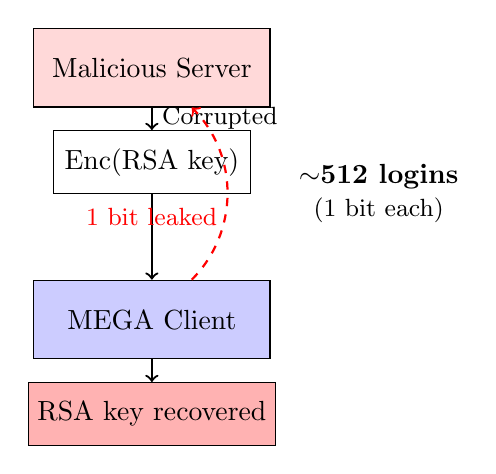
\begin{tikzpicture}[scale=0.8]
				% Server
				\node[draw, rectangle, minimum width=3cm, minimum height=1cm, fill=red!15] (server) at (0,4) {Malicious Server};

				% Client
				\node[draw, rectangle, minimum width=3cm, minimum height=1cm, fill=blue!20] (client) at (0,0) {MEGA Client};

				% Encrypted RSA key
				\node[draw, rectangle, minimum width=2.5cm, minimum height=0.8cm] (enckey) at (0,2.5) {Enc(RSA key)};

				% Attack flow
				\draw[->, thick] (server) -- node[right] {\small Corrupted} (enckey);
				\draw[->, thick] (enckey) -- (client);

				% Oracle feedback
				\draw[->, thick, dashed, red] (client) to[bend right=45] node[left, yshift=-0.3cm] {\small 1 bit leaked} (server);

				% Result
				\node[draw, rectangle, minimum width=3cm, minimum height=0.8cm, fill=red!30] (result) at (0,-1.5) {RSA key recovered};
				\draw[->, thick] (client) -- (result);

				% Attack count
				\node[align=center] at (3.6,2) {\textbf{${\sim}$512 logins}\\{\small (1 bit each)}};
			\end{tikzpicture}
		\end{column}
	\end{columns}
\end{frame}

\begin{frame}{Attack 1: high-level overview}
	\begin{itemize}
		\item \textbf{Threat model:} a malicious service provider controls MEGA's infrastructure
		\item \textbf{Attack strategy:}
		      \begin{enumerate}
			      \item Modify the encrypted RSA private key (no integrity protection)
			      \item Use the client's decryption of the session ID as an oracle
			      \item Binary-search for one of the RSA primes, $q$
		      \end{enumerate}
		\item \textbf{Key insight:} the RSA-CRT implementation leaks information
		      \begin{itemize}
			      \item With a corrupted key, decryption is correct for $m < q$ and garbled for $m \geq q$
			      \item Observable through the session ID the client sends back
		      \end{itemize}
		\item \textbf{Attack cost:} each login leaks one bit of $q$
		      \begin{itemize}
			      \item $q$ has 1024 bits, so a plain binary search needs ${\sim}$1023 logins
			      \item But half the bits of a prime factor suffice: lattice methods (Coppersmith) finish the job $\Rightarrow$ ${\sim}$512 logins\footnote{Later improved to 6 logins by Ryan and Heninger, then to 2: \url{https://appliedcryptography.page/paper/\#mega-recovery}}
		      \end{itemize}
	\end{itemize}
\end{frame}

\begin{frame}{Quick reminder: what does $x^{-1}$ mean?}
	\begin{columns}[c]
		\begin{column}{0.5\textwidth}
			\textbf{In modular arithmetic:}
			\begin{itemize}
				\item $x^{-1}$ is the \textbf{modular inverse} of $x$
				\item It's the number that, when multiplied by $x$, gives 1
				\item $x \cdot x^{-1} \equiv 1 \pmod{n}$
			\end{itemize}
			\vspace{0.5em}
			\textbf{Example:}
			\begin{itemize}
				\item If $x = 3$ and $n = 7$
				\item Then $x^{-1} = 5$ because $3 \cdot 5 = 15 \equiv 1 \pmod{7}$
				\item MEGA's RSA keys store exactly such a value: $u = q^{-1} \bmod p$
			\end{itemize}
		\end{column}
		\begin{column}{0.5\textwidth}
			\textbf{In exponents:}
			\begin{itemize}
				\item Writing $A^{1/r}$ means raising $A$ to $r^{-1}$, computed modulo the group order
				\item $(A^{r})^{1/r} = A^{r \cdot r^{-1}} = A^{1} = A$
				\item Raising to $r$, then to $r^{-1}$, cancels out
			\end{itemize}
			\vspace{0.5em}
			\begin{alertblock}{Key property}
				$((H(x)^{r})^{k})^{1/r} = H(x)^{k}$ \\
				Blind, evaluate, unblind: the heart of the OPRF protocols later in this lecture!
			\end{alertblock}
		\end{column}
	\end{columns}
\end{frame}

\begin{frame}{Attack 1: the decryption oracle}
	\begin{columns}[c]
		\begin{column}{0.5\textwidth}
			\begin{itemize}
				\item \textbf{Setup:}
				      \begin{itemize}
					      \item Server sends corrupted RSA key
					      \item Key has modified $u' \neq u = q^{-1} \bmod p$
				      \end{itemize}
				\item \textbf{Oracle mechanism:}
				      \begin{itemize}
					      \item Server chooses message $m$
					      \item Sends encrypted $[m]_{pk}$ as session ID
					      \item Client decrypts with corrupted key
				      \end{itemize}
				\item \textbf{Observable behavior:}
				      \begin{itemize}
					      \item If $m < q$: correct SID (the one the attacker embedded)
					      \item If $m \geq q$: garbled SID
				      \end{itemize}
			\end{itemize}
		\end{column}
		\begin{column}{0.5\textwidth}
			\begin{tikzpicture}[scale=0.8]
				% Binary search visualization
				\node[draw, rectangle, minimum width=4cm, minimum height=0.5cm] (range) at (0,3) {Search range for $q$};

				% Middle point
				\node[draw, circle, fill=yellow!30] (mid) at (0,2) {$m$};
				\draw[->, thick] (range) -- (mid);

				% Oracle
				\node[draw, rectangle, minimum width=3cm, minimum height=0.8cm, fill=blue!20] (oracle) at (0,0.5) {Decryption Oracle};
				\draw[->, thick] (mid) -- (oracle);

				% Decision
				\node[draw, diamond, aspect=2, fill=green!20] (decision) at (0,-1.5) {$m < q?$};
				\draw[->, thick] (oracle) -- (decision);

				% Left and right
				\node[font=\small] at (-2,-3) {$q > m$: upper half};
				\node[font=\small] at (2,-3) {$q \leq m$: lower half};
				\draw[->, thick] (decision) -- (-2,-2.5) node[midway, left, xshift=-3mm] {Yes};
				\draw[->, thick] (decision) -- (2,-2.5) node[midway, right, xshift=3mm] {No};

				% Iteration count
				\node[draw, rectangle, fill=red!20, align=center, font=\small] at (3.4,1.25) {${\sim}$512 logins\\(1 bit each)};
			\end{tikzpicture}
		\end{column}
	\end{columns}
\end{frame}

\begin{frame}{Attack 2: plaintext recovery attack}
	\begin{columns}[c]
		\begin{column}{0.5\textwidth}
			\begin{itemize}
				\item \textbf{Goal:} Decrypt any AES-ECB ciphertext under the master key
				\item \textbf{Impact:}
				      \begin{itemize}
					      \item All node keys (file/folder encryption)
					      \item Ed25519 signing key
					      \item Curve25519 chat key
					      \item Complete confidentiality breach
				      \end{itemize}
				\item \textbf{Attack requirements:}
				      \begin{itemize}
					      \item RSA key from Attack 1
					      \item Ability to modify key ciphertexts
					      \item Control authentication plaintexts
				      \end{itemize}
				\item \textbf{Cost:} one login recovers 32 bytes --- one full node key
			\end{itemize}
		\end{column}
		\begin{column}{0.5\textwidth}
			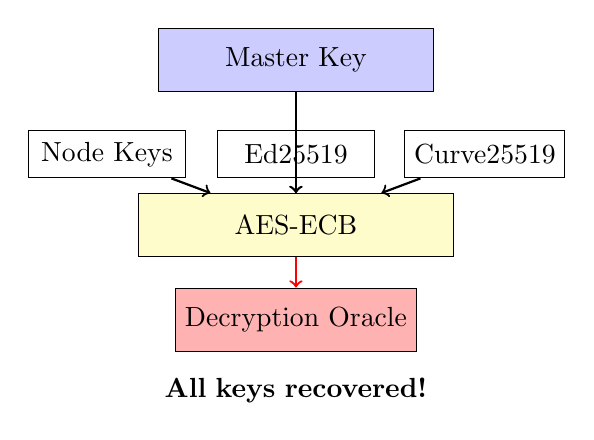
\begin{tikzpicture}[scale=0.6]
				\node[draw, rectangle, minimum width=3.5cm, minimum height=0.8cm, fill=blue!20] (master) at (0,4) {Master Key};

				% Encrypted items
				\node[draw, rectangle, minimum width=2cm, minimum height=0.6cm] (nodekeys) at (-4,2) {Node Keys};
				\node[draw, rectangle, minimum width=2cm, minimum height=0.6cm] (ed25519) at (0,2) {Ed25519};
				\node[draw, rectangle, minimum width=2cm, minimum height=0.6cm] (curve25519) at (4,2) {Curve25519};

				% AES-ECB
				\node[draw, rectangle, minimum width=4cm, minimum height=0.8cm, fill=yellow!20] (aesecb) at (0,0.5) {AES-ECB};

				\draw[->, thick] (master) -- (aesecb);
				\draw[->, thick] (nodekeys) -- (aesecb);
				\draw[->, thick] (ed25519) -- (aesecb);
				\draw[->, thick] (curve25519) -- (aesecb);

				% Attack
				\node[draw, rectangle, minimum width=3cm, minimum height=0.8cm, fill=red!30] (attack) at (0,-1.5) {Decryption Oracle};
				\draw[->, thick, red] (aesecb) -- (attack);

				% Result
				\node[text width=4cm, align=center] at (0,-3) {\textbf{All keys recovered!}};
			\end{tikzpicture}
		\end{column}
	\end{columns}
\end{frame}

\begin{frame}{MEGA's patches: a cautionary tale}
	\begin{itemize}
		\item \textbf{MEGA's response (2022):} not the recommended redesign, but ``sanity checks'' on the decrypted RSA key, plus detailed error reporting when a check fails
		\item \textbf{Follow-up paper (Eurocrypt 2023):} ``Caveat Implementor! Key Recovery Attacks on MEGA''\footnote{\url{https://appliedcryptography.page/paper/\#mega-recovery}}
		      \begin{itemize}
			      \item The new sanity checks and their error messages are themselves a new oracle
			      \item Combined with an AES-ECB \textit{encryption} oracle hiding in the MEGAdrop feature, they yield two new RSA key recovery attacks against the \textit{patched} client
			      \item Slower (${\sim}2^{11}$ logins for the full key), but key recovery all the same
			      \item Side result: the original attack on the unpatched client needs only 2 logins
		      \end{itemize}
		\item \textbf{The irony:} ad-hoc fixes to an ad-hoc design created the next vulnerability
		\item \textbf{Contrast with Nextcloud:} pulled the affected feature and redesigned (coming up)
		\item \textbf{Lesson:} band-aid fixes to broken crypto are dangerous!
	\end{itemize}
\end{frame}

\begin{frame}{MEGA attacks: summary}
	\begin{center}
		\textbf{Note: Due to time constraints, we won't dive into the details of each attack}
	\end{center}
	\begin{columns}[c]
		\begin{column}{0.5\textwidth}
			\begin{itemize}
				\item \textbf{Attack 1 (RSA Key Recovery):} Exploit missing integrity protection to recover the RSA private key in ${\sim}$512 logins
				\item \textbf{Attack 2 (Plaintext Recovery):} Use the recovered RSA key as an AES-ECB decryption oracle for all wrapped keys
				\item \textbf{Attack 3a (Framing):} Forge files via the decryption oracle to frame users with malicious content
			\end{itemize}
		\end{column}
		\begin{column}{0.5\textwidth}
			\begin{itemize}
				\item \textbf{Attack 3b (Integrity):} Forge files with no oracle at all, from one known plaintext/ciphertext block under the master key (e.g., from a public share link)
				\item \textbf{Attack 4 (RSA Decryption):} Bleichenbacher-style padding oracle on MEGA's homebrew RSA padding; ${\sim}2^{17}$ logins, so mostly theoretical
			\end{itemize}
		\end{column}
	\end{columns}
\end{frame}

\begin{frame}{MEGA attacks: at a glance}
	\begin{columns}[c]
		\begin{column}{1\textwidth}
			\begin{table}
				\centering
				\small
				\begin{tabular}{|l|c|c|l|}
					\hline
					\textbf{Attack}    & \textbf{Logins}         & \textbf{Prerequisites} & \textbf{Impact}             \\
					\hline
					RSA Key Recovery   & ${\sim}$512 (later 2)   & None                   & Share keys compromised      \\
					\hline
					Plaintext Recovery & 1 per 32 bytes          & Attack 1               & All keys compromised        \\
					\hline
					Integrity Attack A & 1                       & Attack 2               & File forgery                \\
					\hline
					Integrity Attack B & 1                       & One known AES block    & File forgery                \\
					\hline
					RSA Decryption     & ${\sim}2^{17}$          & None                   & One chat/node key           \\
					\hline
				\end{tabular}
			\end{table}
			\vspace{0.3cm}
			\textbf{Root causes:}
			\begin{itemize}
				\item No authenticated encryption (AES-ECB without a MAC)
				\item Key reuse across different contexts
				\item Homebrew RSA padding instead of OAEP
				\item \textbf{Complex, ad-hoc design without formal analysis!}
			\end{itemize}
		\end{column}
	\end{columns}
\end{frame}

\subsection{Attacks on Nextcloud}

\begin{frame}{Nextcloud: overview}
	\begin{columns}[c]
		\begin{column}{0.75\textwidth}
			\begin{itemize}
				\item Open-source self-hosted cloud storage platform
				\item Founded in 2016 (fork of ownCloud)
				\item \textbf{Key statistics:}
				      \begin{itemize}
					      \item 20+ million users (2017)
					      \item 400,000+ deployments (2022)
					      \item Used by German government, Amnesty International
				      \end{itemize}
				\item \textbf{E2EE claims:}
				      \begin{itemize}
					      \item ``Zero Knowledge'' server
					      \item Secure against full server breach
					      \item Enterprise-grade encryption
				      \end{itemize}
			\end{itemize}
		\end{column}
		\begin{column}{0.25\textwidth}
			\imagewithcaption{nextcloud-logo.png}{Nextcloud's logo.}
		\end{column}
	\end{columns}
\end{frame}

\begin{frame}{Nextcloud: E2EE design}
	\begin{columns}[c]
		\begin{column}{0.6\textwidth}
			\begin{itemize}
				\item E2EE is \textbf{off by default}; users mark folders as E2EE
				\item \textbf{Mnemonic} (12 words, client-generated, user stores it) $\rightarrow$ master key $\rightarrow$ wraps the RSA private key, stored on the server
				\item \textbf{Metadata key}, one per folder: RSA-OAEP-encrypted to each member's public key; encrypts the folder metadata, i.e., all file keys
				\item \textbf{File key}: random 128-bit AES-GCM key per file
				\item \textbf{Key rotation}: an \textit{array} of metadata keys per folder; the highest index is current
			\end{itemize}
		\end{column}
		\begin{column}{0.4\textwidth}
			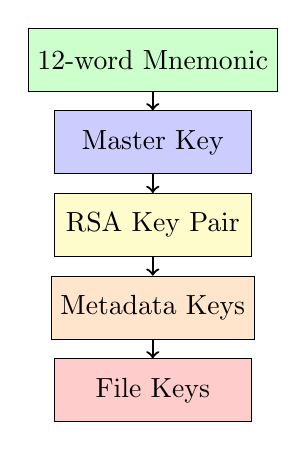
\begin{tikzpicture}[scale=0.7]
				% Mnemonic
				\node[draw, rectangle, minimum width=3cm, minimum height=0.8cm, fill=green!20] (mnemonic) at (0,5) {12-word Mnemonic};

				% Master key
				\node[draw, rectangle, minimum width=2.5cm, minimum height=0.8cm, fill=blue!20] (master) at (0,3.5) {Master Key};
				\draw[->, thick] (mnemonic) -- (master);

				% RSA keys
				\node[draw, rectangle, minimum width=2.5cm, minimum height=0.8cm, fill=yellow!20] (rsa) at (0,2) {RSA Key Pair};
				\draw[->, thick] (master) -- (rsa);

				% Metadata keys
				\node[draw, rectangle, minimum width=2.5cm, minimum height=0.8cm, fill=orange!20] (metadata) at (0,0.5) {Metadata Keys};
				\draw[->, thick] (rsa) -- (metadata);

				% File keys
				\node[draw, rectangle, minimum width=2.5cm, minimum height=0.8cm, fill=red!20] (filekeys) at (0,-1) {File Keys};
				\draw[->, thick] (metadata) -- (filekeys);
			\end{tikzpicture}
		\end{column}
	\end{columns}
\end{frame}

\begin{frame}{Nextcloud vulnerabilities: overview}
	\begin{columns}[c]
		\begin{column}{1\textwidth}
			\textbf{Three vulnerabilities, found by Albrecht, Backendal, Coppola and Paterson (2024):}\footnote{\url{https://appliedcryptography.page/paper/\#nextcloud-break}}
			\begin{enumerate}
				\item \textbf{Key insertion attack}
				      \begin{itemize}
					      \item The server substitutes a metadata key of its own choosing
					      \item Exploits the fact that RSA-OAEP says nothing about \textit{who} encrypted
				      \end{itemize}
				\item \textbf{Ghost key attack}
				      \begin{itemize}
					      \item The server makes the client index past the end of the key array
					      \item The default entry is an all-zero key
				      \end{itemize}
				\item \textbf{Nonce reuse in AES-GCM}
				      \begin{itemize}
					      \item A modified file is re-encrypted under the same key \textit{and} the same nonce
					      \item Plaintext recovery and forgery follow
				      \end{itemize}
			\end{enumerate}
			\vspace{0.2cm}
			Each one, on its own, lets a malicious server read and modify every file.
		\end{column}
	\end{columns}
\end{frame}

\begin{frame}{Attack 1: key insertion attack}
	\begin{columns}[c]
		\begin{column}{0.7\textwidth}
			\begin{itemize}
				\item \textbf{Root cause:} RSA-OAEP provides confidentiality but \textbf{not authentication}
				\item \textbf{Attack scenario:}
				      \begin{enumerate}
					      \item Server creates chosen metadata key
					      \item Encrypts it with user's RSA public key
					      \item Places ciphertext in user's folder
					      \item Triggers key rotation
				      \end{enumerate}
				\item \textbf{Impact:}
				      \begin{itemize}
					      \item Server knows metadata key
					      \item Can decrypt all file keys
					      \item Can insert/modify files
				      \end{itemize}
			\end{itemize}
		\end{column}
		\begin{column}{0.3\textwidth}
			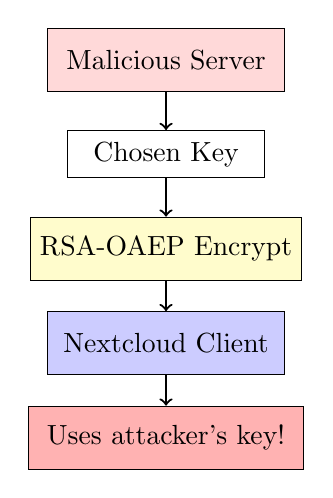
\begin{tikzpicture}[scale=0.8]
				% Malicious server
				\node[draw, rectangle, minimum width=3cm, minimum height=0.8cm, fill=red!15] (server) at (0,4) {Malicious Server};

				% Chosen key
				\node[draw, rectangle, minimum width=2.5cm, minimum height=0.6cm] (chosenkey) at (0,2.5) {Chosen Key};
				\draw[->, thick] (server) -- (chosenkey);

				% RSA-OAEP
				\node[draw, rectangle, minimum width=3cm, minimum height=0.8cm, fill=yellow!20] (rsaoaep) at (0,1) {RSA-OAEP Encrypt};
				\draw[->, thick] (chosenkey) -- (rsaoaep);

				% Client
				\node[draw, rectangle, minimum width=3cm, minimum height=0.8cm, fill=blue!20] (client) at (0,-0.5) {Nextcloud Client};
				\draw[->, thick] (rsaoaep) -- (client);

				% Result
				\node[draw, rectangle, minimum width=3.5cm, minimum height=0.8cm, fill=red!30] (result) at (0,-2) {Uses attacker's key!};
				\draw[->, thick] (client) -- (result);
			\end{tikzpicture}
		\end{column}
	\end{columns}
\end{frame}

\begin{frame}{The authentication problem in public key encryption}
	\begin{columns}[c]
		\begin{column}{1\textwidth}
			\begin{itemize}
				\item \textbf{What RSA-OAEP provides:}
				      \begin{itemize}
					      \item Confidentiality: Only private key holder can decrypt
					      \item Chosen-ciphertext security (IND-CCA2)
				      \end{itemize}
				\item \textbf{What RSA-OAEP does NOT provide:}
				      \begin{itemize}
					      \item Authentication: No proof of who created the ciphertext
					      \item Anyone with the public key can encrypt
				      \end{itemize}
				\item \textbf{Nextcloud's assumption:}
				      \begin{itemize}
					      \item ``Only legitimate users will encrypt metadata keys''
					      \item But server has all public keys!
				      \end{itemize}
				\item \textbf{Solution approaches:}
				      \begin{itemize}
					      \item Digital signatures on encrypted keys
					      \item Authenticated encryption (e.g., signcryption)
					      \item Key exchange protocols instead of PKE
				      \end{itemize}
			\end{itemize}
		\end{column}
	\end{columns}
\end{frame}

\begin{frame}{Attack 2: ghost key attack}
	\begin{columns}[c]
		\begin{column}{0.5\textwidth}
			\begin{itemize}
				\item \textbf{Vulnerability:} Missing bounds checking on metadata key array
				\item \textbf{Attack mechanism:}
				      \begin{enumerate}
					      \item Server modifies key index
					      \item Points to non-existent entry
					      \item Client allocates default key
					      \item Default is all zeros!
				      \end{enumerate}
				\item \textbf{Result:}
				      \begin{itemize}
					      \item Files encrypted with known key (\texttt{0x00...})
					      \item Complete confidentiality loss
					      \item Trivial file forgery
				      \end{itemize}
			\end{itemize}
		\end{column}
		\begin{column}{0.5\textwidth}
			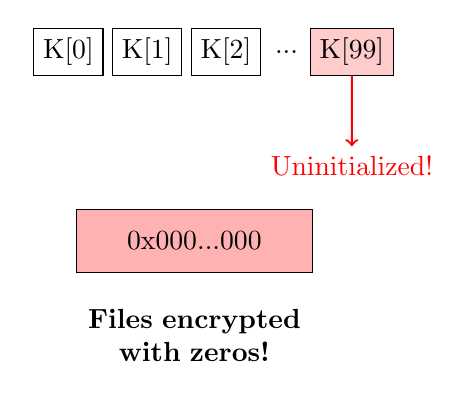
\begin{tikzpicture}[scale=0.8]
				% Key array
				\node[draw, rectangle, minimum width=0.8cm, minimum height=0.6cm] (key0) at (0,3) {K[0]};
				\node[draw, rectangle, minimum width=0.8cm, minimum height=0.6cm] (key1) at (1.25,3) {K[1]};
				\node[draw, rectangle, minimum width=0.8cm, minimum height=0.6cm] (key2) at (2.5,3) {K[2]};
				\node[right] at (3.125,3) {...};

				% Invalid index
				\node[draw, rectangle, minimum width=0.8cm, minimum height=0.6cm, fill=red!20] (keyX) at (4.5,3) {K[99]};

				% Arrow to ghost
				\draw[->, thick, red] (keyX) -- (4.5,1.5) node[below] {Uninitialized!};

				% All zeros
				\node[draw, rectangle, minimum width=3cm, minimum height=0.8cm, fill=red!30] (zeros) at (2,0) {0x000...000};

				% Result
				\node[text width=4cm, align=center] at (2,-1.5) {\textbf{Files encrypted with zeros!}};
			\end{tikzpicture}
		\end{column}
	\end{columns}
\end{frame}

\begin{frame}{Attack 3: nonce reuse in AES-GCM}
	\begin{columns}[c]
		\begin{column}{0.6\textwidth}
			\begin{itemize}
				\item \textbf{Critical flaw:} Same nonce used when file is modified
				\item \textbf{AES-GCM requirement:} Never reuse nonce with same key
				\item \textbf{Consequences of nonce reuse:}
				      \begin{itemize}
					      \item Keystream repeats
					      \item XOR of plaintexts revealed
					      \item Authentication key recovery
				      \end{itemize}
				\item \textbf{Attack scenarios:}
				      \begin{itemize}
					      \item \textbf{Plaintext recovery:} two versions of one file suffice
					      \item \textbf{Forgery:} recover the GCM key, inject files
				      \end{itemize}
			\end{itemize}
		\end{column}
		\begin{column}{0.4\textwidth}
			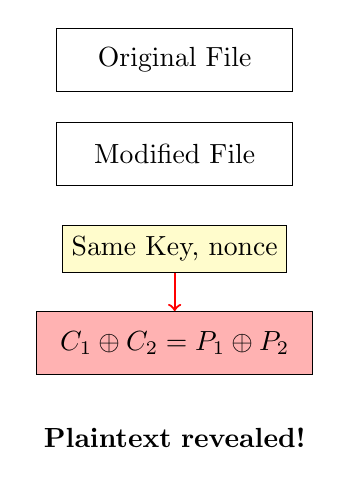
\begin{tikzpicture}[scale=0.8]
				% Original file
				\node[draw, rectangle, minimum width=3cm, minimum height=0.8cm] (file1) at (0,3) {Original File};

				% Modified file
				\node[draw, rectangle, minimum width=3cm, minimum height=0.8cm] (file2) at (0,1.5) {Modified File};

				% Same key and nonce
				\node[draw, rectangle, minimum width=2.5cm, minimum height=0.6cm, fill=yellow!20] (keyiv) at (0,0) {Same Key, nonce};

				% XOR reveals difference
				\node[draw, rectangle, minimum width=3.5cm, minimum height=0.8cm, fill=red!30] (xor) at (0,-1.5) {$C_1 \oplus C_2 = P_1 \oplus P_2$};
				\draw[->, thick, red] (keyiv) -- (xor);

				% Result
				\node[text width=3.5cm, align=center] at (0,-3) {\textbf{Plaintext revealed!}};
			\end{tikzpicture}
		\end{column}
	\end{columns}
\end{frame}

\begin{frame}{Nextcloud's response}
	\begin{itemize}
		\item \textbf{Disclosure:} January 2, 2023; Nextcloud confirmed within ten days; patches for all three vulnerabilities on March 29, 2023, each with a CVE
		\item \textbf{Ghost key and nonce reuse:} straightforward implementation fixes (a bounds check; a fresh nonce on every re-encryption)
		\item \textbf{Key insertion:} no such quick fix --- the design had no notion of \textit{who} encrypted a metadata key
		      \begin{itemize}
			      \item Stop-gap: a checksum over the metadata keys, derived from the user's own mnemonic
			      \item Only the owner can verify it, so \textbf{E2EE file sharing was disabled} until a redesign
			      \item A significant revision of the cryptographic design later restored sharing
		      \end{itemize}
		\item \textbf{Lesson:} authentication is as important as confidentiality --- and much harder to retrofit
	\end{itemize}
\end{frame}

\begin{frame}{Comparing MEGA and Nextcloud failures}
	\begin{columns}
		\begin{column}{0.5\textwidth}
			\textbf{MEGA}
			\vspace{0.3cm}
			\begin{itemize}
				\item No authenticated encryption
				\item Complex key hierarchy
				\item ECB mode usage
				\item Homebrew RSA padding
				\item Patches introduced new flaws
			\end{itemize}
		\end{column}
		\begin{column}{0.5\textwidth}
			\textbf{Nextcloud}
			\vspace{0.3cm}
			\begin{itemize}
				\item Missing authentication
				\item Implementation bugs
				\item Nonce reuse in AES-GCM
				\item Bounds checking errors
				\item Had to disable features
			\end{itemize}
		\end{column}
	\end{columns}
	\vspace{0.5cm}
	\begin{center}
		\textbf{Common theme:} Complex, ad-hoc designs without formal security analysis!
	\end{center}
\end{frame}

\subsection{The Rest of the Ecosystem}

\begin{frame}{The rest of the ecosystem (2024)}
	\begin{columns}[c]
		\begin{column}{1\textwidth}
			\begin{itemize}
				\item 2024 (ACM CCS): a systematic analysis of five more E2EE providers --- Sync, pCloud, Icedrive, Seafile, Tresorit\footnote{\url{https://appliedcryptography.page/paper/\#cloud-broken}}
				\item Collectively serving 22+ million users
				\item \textbf{Key finding:} the same failures, rediscovered independently by each vendor
				\item \textbf{Common patterns:}
				      \begin{itemize}
					      \item Unauthenticated key material (Sync, pCloud)
					      \item Unauthenticated encryption modes (Icedrive, Seafile)
					      \item Missing integrity protection on file chunks
					      \item Protocol downgrade attacks
				      \end{itemize}
				\item \textbf{Impact:} four of the five fail basic security requirements against a malicious server
			\end{itemize}
		\end{column}
	\end{columns}
\end{frame}

\begin{frame}{Attack highlights across five providers}
	\begin{columns}[c]
		\begin{column}{0.5\textwidth}
			\begin{itemize}
				\item \textbf{Key replacement attacks}
				      \begin{itemize}
					      \item Sync/pCloud: No authentication of material encrypted under public keys
					      \item Server replaces user keys with attacker-controlled keys
					      \item All future uploads compromised
				      \end{itemize}
			\end{itemize}
			\vspace{0.3cm}
			\begin{itemize}
				\item \textbf{Protocol downgrade (Seafile)}
				      \begin{itemize}
					      \item Server forces the client back to a deprecated key derivation
					      \item OpenSSL's \texttt{EVP\_BytesToKey}: 3 rounds of SHA-1 instead of PBKDF2
					      \item Enables offline password cracking
				      \end{itemize}
			\end{itemize}
		\end{column}
		\begin{column}{0.5\textwidth}
			\begin{itemize}
				\item \textbf{Link sharing leakage (Sync)}
				      \begin{itemize}
					      \item Password embedded in URL path
					      \item Sent to server on every click
					      \item Complete confidentiality breach
				      \end{itemize}
			\end{itemize}
			\vspace{0.3cm}
			\begin{itemize}
				\item \textbf{Unauthenticated chunking}
				      \begin{itemize}
					      \item Seafile/pCloud: Can reorder/remove file chunks
					      \item Icedrive: Twofish-CBC allows controlled tampering
					      \item Files corrupted without detection
				      \end{itemize}
			\end{itemize}
		\end{column}
	\end{columns}
\end{frame}

\begin{frame}{The state of E2EE cloud storage: a broken ecosystem}
	\begin{columns}[c]
		\begin{column}{1\textwidth}
			\begin{itemize}
				\item \textbf{Systemic failures across providers:}
				      \begin{itemize}
					      \item 4 out of 5 analyzed providers have critical vulnerabilities
					      \item Tresorit fared best: only metadata tampering and a limited public-key substitution issue
					      \item The same mistakes, made independently, by companies that never talked to each other
				      \end{itemize}
				\item \textbf{Root causes echo MEGA and Nextcloud:}
				      \begin{itemize}
					      \item Ad-hoc designs that misunderstand what a primitive guarantees (encryption $\neq$ integrity, PKE $\neq$ authentication)
					      \item Nobody wrote down a threat model with a malicious server in it
				      \end{itemize}
				\item \textbf{Key lesson:} E2EE cloud storage is not a ``solved problem'' --- it is a problem the industry solved wrong, five times
			\end{itemize}
		\end{column}
	\end{columns}
\end{frame}

\begin{frame}{Discussion time}
	\begin{columns}[c]
		\begin{column}{0.8\textwidth}
			\begin{enumerate}
				\item \textbf{Which of the attacks you just saw need a \textit{malicious} server?}
				      \begin{itemize}
					      \item Which would also work for an outsider who breached the server once and walked off with its database?
				      \end{itemize}
				\item \textbf{MEGA could not simply rotate everyone's keys. Why not?}
				      \begin{itemize}
					      \item Hint: who holds the only means of decrypting the master key?
				      \end{itemize}
				\item \textbf{Nextcloud pulled a feature; MEGA added checks.} Which response would you rather have as a user? As the engineer on call?
				\item \textbf{Both MEGA and Nextcloud used RSA encryption to hand out keys.} What property were they assuming that public-key encryption simply does not provide?
			\end{enumerate}
		\end{column}
	\end{columns}
\end{frame}

\section{Authentication: Beyond Password Hashing}

\begin{frame}{Beyond password hashing: PAKEs}
	\begin{itemize}
		\item With password hashing, the server \textit{sees your password} at every login --- TLS protects it in transit, then the server hashes it
		      \begin{itemize}
			      \item A malicious or compromised server can simply log passwords as they arrive
			      \item And a stolen hash database is an offline dictionary attack waiting to happen (salts and memory-hard functions slow it down; they don't stop it)
		      \end{itemize}
		\item \textbf{Password-authenticated key exchange (PAKE)}, sometimes marketed as ``zero-knowledge password proofs'':
		      \begin{itemize}
			      \item The server never sees the password --- not at login, not even at registration
			      \item An eavesdropper, or a fake server, learns nothing it can attack offline
			      \item Both sides end up with a shared session key --- handy for E2EE storage
		      \end{itemize}
		\item Two examples: \textbf{SRP} (1998, deployed everywhere) and \textbf{OPAQUE} (2018, the modern one)
	\end{itemize}
\end{frame}

\begin{frame}{SRP (Secure Remote Password)}
	\begin{itemize}
		\item Developed by Tom Wu at Stanford (1998)
		\item \textbf{Key properties:}
		      \begin{itemize}
			      \item Password never transmitted, even encrypted
			      \item Mutual authentication between client and server
			      \item Generates session key for subsequent encryption
			      \item Patent-free and standardized (RFC 2945)
		      \end{itemize}
		\item \textbf{How it works:}
		      \begin{itemize}
			      \item Registration: Client sends verifier derived from password
			      \item Authentication: Zero-knowledge proof using verifier
			      \item Based on discrete logarithm problem
		      \end{itemize}
		\item \textbf{Adoption:} Used by Apple iCloud, 1Password, and ProtonMail
	\end{itemize}
\end{frame}

\begin{frame}{SRP: how it works, visually}
	\begin{center}
		\begin{tikzpicture}[
				scale=0.85, transform shape,
				actor/.style={draw, rounded corners, minimum width=2.8cm, minimum height=0.62cm, font=\small\bfseries},
				note/.style={draw, rounded corners, align=center, font=\scriptsize, inner sep=3.5pt},
				stepnum/.style={circle, fill=cipherprimary, text=cipherwhite, font=\bfseries\scriptsize, inner sep=1.2pt, minimum size=0.42cm},
				band/.style={rounded corners, draw=ciphergraydark, thick},
				msg/.style={->, very thick}
			]
			% Phase bands (drawn first, everything else on top)
			\draw[band, fill=ciphergray] (-2.95,-0.42) rectangle (11.15,-2.28);
			\draw[band, fill=ciphergray] (-2.95,-2.42) rectangle (11.15,-6.45);
			\node[rotate=90, font=\tiny\bfseries, text=cipherprimary] at (-2.7,-1.35) {SIGN-UP (once)};
			\node[rotate=90, font=\tiny\bfseries, text=cipherprimary] at (-2.7,-4.4) {LOGIN (every time)};

			% Lifelines and actors
			\draw[dashed, gray] (0,-0.31) -- (0,-6.45);
			\draw[dashed, gray] (9,-0.31) -- (9,-6.45);
			\node[actor, fill=blue!15] (alice) at (0,0) {Alice's device};
			\node[actor, fill=red!15] (server) at (9,0) {Server};
			\node[font=\tiny, text=gray] at (4.5,0) {public: prime $N$, generator $g$, $k = H(N, g)$; all math mod $N$};

			% Step 1: password -> verifier
			\node[stepnum] at (-2.05,-1.18) {1};
			\node[note, fill=blue!12] at (0,-1.18) {picks salt, computes\\$x = H(\mathrm{salt}, pw)$,\\verifier $v = g^x$};
			\node[note, fill=red!12] at (9,-1.18) {stores $(\mathrm{salt}, v)$:\\can \emph{verify} Alice, but\\inverting $g^x$ is infeasible};

			% Step 2: send verifier
			\node[stepnum] at (-2.05,-1.98) {2};
			\draw[msg, cipherprimary] (0,-1.98) -- node[above, font=\scriptsize] {$\mathrm{salt},\ v = g^x$}
			node[below, font=\tiny, text=red!70!black] {neither $pw$ nor $x$ is ever sent} (9,-1.98);

			% Step 3: exchange ephemeral DH values
			\node[stepnum] at (-2.05,-3.28) {3};
			\draw[msg, cipherprimary] (0,-2.95) -- node[above, font=\scriptsize] {$A = g^a$ \ (fresh secret exponent $a$)} (9,-2.95);
			\draw[msg, cipherprimary] (9,-3.62) -- node[above, font=\scriptsize] {$\mathrm{salt},\ B = kv + g^b$ \ (fresh secret exponent $b$)} (0,-3.62);
			\node[font=\tiny, text=cipherprimary] at (4.5,-3.88) {both sides compute $u = H(A, B)$};

			% Step 4: both derive the shared secret
			\node[stepnum] at (-2.05,-4.42) {4};
			\node[note, fill=blue!12] (mixa) at (0,-4.42) {$x = H(\mathrm{salt}, pw)$\\$S = (B - kg^x)^{\,a + ux}$\\$K = H(S)$};
			\node[note, fill=red!12] (mixs) at (9,-4.42) {$S = (A \cdot v^u)^{\,b}$\\$K = H(S)$};
			\node[note, fill=cipherprimarylight!45, font=\scriptsize] (samek) at (4.5,-4.42) {\textbf{the same $K$!}\\{\tiny both $S = g^{\,b(a + ux)}$}};
			\draw[<->, thick, ciphersecondary] (mixa.east) -- (samek.west);
			\draw[<->, thick, ciphersecondary] (samek.east) -- (mixs.west);

			% Step 5: mutual proof
			\node[stepnum] at (-2.05,-5.38) {5};
			\draw[<->, very thick, ciphersecondary] (0,-5.38) -- node[above, font=\scriptsize] {proofs: $M_1 = H(A, B, K)$, $M_2 = H(A, M_1, K)$}
			node[below, font=\tiny, text=red!70!black] {wrong password? the $K$'s don't match, proofs fail, login rejected} (9,-5.38);

			% Eavesdropper note
			\node[note, fill=cipherwhite, font=\tiny, text width=9.6cm] at (4.5,-6.13) {\textbf{Eve on the wire?} Recovering $a$ or $b$ from $A$ and $B$ means solving\\the discrete log problem; without $pw$ or $v$, she cannot compute $S$.};
		\end{tikzpicture}
	\end{center}
\end{frame}

\begin{frame}{Discrete logarithm problem}{Reminder}
	\begin{itemize}
		\item The discrete logarithm problem:
		      \begin{itemize}
			      \item Given a finite cyclic group $G$, a generator $g \in G$, and an element
			            $h \in G$, find the integer $x$ such that $g^{x}=h$
		      \end{itemize}
		\item In more concrete terms:
		      \begin{itemize}
			      \item Let $p$ be a large prime and let $g$ be a generator of the multiplicative
			            group $\mathbb{Z}_{p}^{*}$ (all nonzero integers modulo $p$).
			      \item Given:
			            \begin{itemize}
				            \item $g \in \mathbb{Z}_{p}^{*}$, $h \in \mathbb{Z}_{p}^{*}$

				            \item Find $x \in \{0, 1, \ldots, p-2\}$ such that $g^{x} \equiv h \pmod
					                  {p}$
			            \end{itemize}
			      \item This problem is believed to be computationally hard when $p$ is large
			            and $g$ is a primitive root modulo $p$.
			            \begin{itemize}
				            \item ``Believed to be'' = we don't know of any way to do it that doesn't
				                  take forever, unless we have a large-scale, fault-tolerant quantum computer (Shor's
				                  algorithm)
			            \end{itemize}
		      \end{itemize}
	\end{itemize}
\end{frame}

\begin{frame}{OPAQUE: next-generation password authentication}
	\begin{itemize}
		\item Developed by Jarecki, Krawczyk, and Xu (2018)
		\item \textbf{Advantages over SRP:}
		      \begin{itemize}
			      \item Stronger security proofs in UC framework
			      \item Protection against pre-computation attacks
		      \end{itemize}
		\item \textbf{Key innovation:} Oblivious PRF (OPRF)
		      \begin{itemize}
			      \item Server helps compute PRF without learning input
			      \item Prevents server from testing password guesses
		      \end{itemize}
		\item Standardized in 2025 as RFC 9807 (OPRF component: RFC 9497)
		\item Early adoption by WhatsApp for backup encryption (2021)
	\end{itemize}
\end{frame}

\begin{frame}{OPAQUE: how it works under the hood}
	\begin{columns}[c]
		\begin{column}{1\textwidth}
			\begin{itemize}
				\item \textbf{OPAQUE combines three key components:}
				      \begin{itemize}
					      \item \textbf{OPRF (Oblivious PRF):} the server helps compute a function of the password without seeing it
					      \item \textbf{Authenticated key exchange:} derives session keys once the password checks out
					      \item \textbf{Password hardening:} a slow, memory-hard hash makes every guess expensive
				      \end{itemize}
				\item \textbf{The magic:} the server stores a ``password file'' per user, but:
				      \begin{itemize}
					      \item It contains no password and no password hash
					      \item In the protocol, the server only ever sees \textit{blinded} values --- nothing it can test a guess against
					      \item The client proves knowledge of the password without revealing it
					            \begin{itemize}
						            \item You could even say they perform a \textit{zero-knowledge proof}!
					            \end{itemize}
				      \end{itemize}
			\end{itemize}
		\end{column}
	\end{columns}
\end{frame}

\begin{frame}{What is an OPRF?}{Oblivious Pseudorandom Function}
	\begin{columns}[c]
		\begin{column}{1\textwidth}
			\begin{itemize}
				\item \textbf{Definition:} A two-party protocol where:
				      \begin{itemize}
					      \item Client has input $x$
					      \item Server has key $k$
					      \item Client learns $F(k, x)$ and nothing else
					      \item Server learns nothing about $x$
					            \begin{itemize}
						            \item You could even say they perform a \textit{multi-party computation}!
					            \end{itemize}
				      \end{itemize}
				\item \textbf{Key properties:}
				      \begin{itemize}
					      \item \textbf{Oblivious:} Server doesn't learn client's input
					      \item \textbf{Verifiable (VOPRF variant):} Client can verify correct computation
					      \item \textbf{Deterministic:} Same input always gives the same output
				      \end{itemize}
			\end{itemize}
		\end{column}
	\end{columns}
\end{frame}

\begin{frame}{OPAQUE registration: step by step}
	\begin{columns}[c]
		\begin{column}{0.5\textwidth}
			\textbf{Client actions:}
			\begin{enumerate}
				\item Choose password $pw$
				\item Run OPRF with server:\footnote{The OPRF runs in a cyclic group $\mathbb{G}$ of prime order $q$, with blinding factor $r \twoheadleftarrow \mathbb{Z}_q$ and server OPRF key $k$. This is (lightly simplified) 2HashDH, covered in detail at the end of this lecture; full OPAQUE also hardens $rwd$ with a slow, memory-hard hash.}
				      \begin{itemize}
					      \item Send blinded $H(pw)^r$
					      \item Get back $(H(pw)^r)^k$
					      \item Unblind: $rwd = ((H(pw)^r)^k)^{1/r} = H(pw)^k$
				      \end{itemize}
				\item Generate random private key $sk_c$
				\item Encrypt: $env = \text{Enc}(rwd, sk_c)$
				\item Send $(env, pk_c)$ to server
			\end{enumerate}
		\end{column}
		\begin{column}{0.5\textwidth}
			\textbf{Server actions:}
			\begin{enumerate}
				\item Generate OPRF key $k$
				\item Respond to OPRF:
				      \begin{itemize}
					      \item Receive blinded value
					      \item Return $(\text{blinded})^k$
				      \end{itemize}
				\item Generate key pair $(sk_s, pk_s)$
				\item Store password file:
				      \begin{itemize}
					      \item Client's $env$ (encrypted)
					      \item Client's $pk_c$
					      \item Own $sk_s, pk_s$
					      \item OPRF key $k$
				      \end{itemize}
			\end{enumerate}
		\end{column}
	\end{columns}
\end{frame}

\begin{frame}{What's in the password file?}
	\begin{columns}[c]
		\begin{column}{0.6\textwidth}
			\begin{itemize}
				\item \textbf{Client's envelope ($env$):}
				      \begin{itemize}
					      \item Encrypted with $rwd = H(pw)^k$
					      \item Contains client's private key $sk_c$
					      \item Server can't decrypt without password
				      \end{itemize}
				\item \textbf{Public keys:}
				      \begin{itemize}
					      \item Client's $pk_c$ (for key exchange)
					      \item Server's $pk_s$ (for authentication)
				      \end{itemize}
				\item \textbf{Server's secrets:}
				      \begin{itemize}
					      \item OPRF key $k$ (for password evaluation)
					      \item Server private key $sk_s$
				      \end{itemize}
			\end{itemize}
		\end{column}
		\begin{column}{0.4\textwidth}
			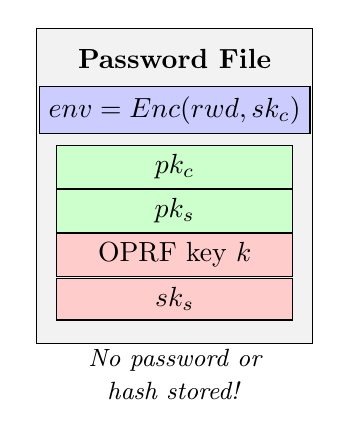
\begin{tikzpicture}[scale=0.8]
				% Password file box
				\node[draw, rectangle, minimum width=3.5cm, minimum height=4cm, fill=gray!10] (file) at (0,0) {};
				\node[above] at (0,1.7) {\textbf{Password File}};

				% Contents
				\node[draw, rectangle, minimum width=3cm, minimum height=0.6cm, fill=blue!20] (env) at (0,1.2) {$env = \text{Enc}(rwd, sk_c)$};
				\node[draw, rectangle, minimum width=3cm, minimum height=0.5cm, fill=green!20] (pkc) at (0,0.3) {$pk_c$};
				\node[draw, rectangle, minimum width=3cm, minimum height=0.5cm, fill=green!20] (pks) at (0,-0.4) {$pk_s$};
				\node[draw, rectangle, minimum width=3cm, minimum height=0.5cm, fill=red!20] (k) at (0,-1.1) {OPRF key $k$};
				\node[draw, rectangle, minimum width=3cm, minimum height=0.5cm, fill=red!20] (sks) at (0,-1.8) {$sk_s$};

				% Note
				\node[text width=3.5cm, align=center] at (0,-3) {\small\textit{No password or hash stored!}};
			\end{tikzpicture}
		\end{column}
	\end{columns}
\end{frame}

\begin{frame}{OPAQUE login (after registration)}
	\begin{columns}[c]
		\begin{column}{0.5\textwidth}
			\begin{itemize}
				\item[1.]\textbf{Client starts OPRF:}
				      \begin{itemize}
					      \item Blinds password: $\alpha = H(pw)^r$
					      \item Sends $\alpha$ to server
					      \item Note: This $r$ is freshly sampled --- different from the one used at registration and at each previous login
				      \end{itemize}
				\item[2.]\textbf{Server responds:}
				      \begin{itemize}
					      \item Computes $\beta = \alpha^k = H(pw)^{rk}$
					      \item Sends back $\beta$ and encrypted envelope $env$
				      \end{itemize}
			\end{itemize}
		\end{column}
		\begin{column}{0.5\textwidth}
			\begin{itemize}
				\item[3.]\textbf{Client recovers private key:}
				      \begin{itemize}
					      \item Unblinds: $rwd = \beta^{1/r} = H(pw)^k$
					      \item Decrypts: $sk_c = \text{Dec}(rwd, env)$
					      \item If the password is wrong, decryption fails!
				      \end{itemize}
				\item[4.]\textbf{Authenticated key exchange:}
				      \begin{itemize}
					      \item Client and server run AKE using their key pairs
					      \item Derives session key and export key
					      \item Mutual authentication achieved
				      \end{itemize}
			\end{itemize}
		\end{column}
	\end{columns}
\end{frame}

\begin{frame}{Can the server test passwords?}
	\begin{columns}[c]
		\begin{column}{0.5\textwidth}
			\textbf{From the protocol: no}
			\begin{itemize}
				\item It sees only $\alpha = H(pw)^r$: a uniformly random group element, fresh each login
				\item Nothing to test a guess against --- same for an eavesdropper or a phishing server
				\item Contrast SRP: the salt is public, so attackers can \textit{pre-compute} a per-user dictionary
			\end{itemize}
		\end{column}
		\begin{column}{0.5\textwidth}
			\textbf{From its own password file: yes, slowly}
			\begin{itemize}
				\item Whoever holds $k$ and $env$ can guess: compute $H(pw')^k$, try to open $env$
				\item Unavoidable for any password scheme --- the server must be able to check the password
				\item OPAQUE's promise: no pre-computation ($k$ is a secret salt); every guess pays for the memory-hard hash
				\item WhatsApp's trick, next: keep $k$ inside an HSM that counts attempts
			\end{itemize}
		\end{column}
	\end{columns}
\end{frame}

\begin{frame}{OPAQUE's security guarantees}
	\begin{columns}[c]
		\begin{column}{0.5\textwidth}
			\textbf{Against server compromise:}
			\begin{itemize}
				\item[\textcolor{green}{\mycheckmark}] No pre-computation: the attacker's dictionary work starts \textit{after} the breach, per user
				\item[\textcolor{green}{\mycheckmark}] Forward secrecy: past session keys stay secret even if $sk_s$ and the password file leak
				\item[\textcolor{red}{$\times$}] Offline guessing against the stolen file is still possible (as in any password scheme)
			\end{itemize}
		\end{column}
		\begin{column}{0.5\textwidth}
			\textbf{Against active attacks:}
			\begin{itemize}
				\item[\textcolor{green}{\mycheckmark}] Mutual authentication and key confirmation
				\item[\textcolor{green}{\mycheckmark}] A fake server learns nothing about the password (unlike a phishing page that asks you to type it)
				\item[\textcolor{green}{\mycheckmark}] Each online guess costs one interaction --- so rate limiting actually works
			\end{itemize}
		\end{column}
	\end{columns}
	\vspace{0.3cm}
	\begin{center}
		\textbf{Bonus:} the client also gets an \textit{export key} nobody else knows --- authentication and key derivation in one protocol!
	\end{center}
\end{frame}

\begin{frame}{Comparing authentication approaches}
	\begin{columns}
		\begin{column}{0.33\textwidth}
			\textbf{Password Hashing}
			\vspace{0.3cm}
			\begin{itemize}
				\item[\textcolor{green}{\mycheckmark}] Simple to implement
				\item[\textcolor{green}{\mycheckmark}] Well understood
				\item[\textcolor{red}{$\times$}] Offline attacks
				\item[\textcolor{red}{$\times$}] Server sees password
			\end{itemize}
		\end{column}
		\begin{column}{0.33\textwidth}
			\textbf{SRP}
			\vspace{0.3cm}
			\begin{itemize}
				\item[\textcolor{green}{\mycheckmark}] No offline attacks by eavesdroppers
				\item[\textcolor{green}{\mycheckmark}] Decades of deployment
				\item[\textcolor{red}{$\times$}] No formal security proof
				\item[\textcolor{red}{$\times$}] Pre-computation attacks
			\end{itemize}
		\end{column}
		\begin{column}{0.34\textwidth}
			\textbf{OPAQUE}
			\vspace{0.3cm}
			\begin{itemize}
				\item[\textcolor{green}{\mycheckmark}] Strongest security
				\item[\textcolor{green}{\mycheckmark}] Forward secrecy
				\item[\textcolor{red}{$\times$}] Standardized only in 2025
				\item[\textcolor{red}{$\times$}] Adoption still ramping up
			\end{itemize}
		\end{column}
	\end{columns}
	\vspace{0.5cm}
	\begin{center}
		\textit{For E2EE storage: Can derive encryption keys from authentication protocol outputs}
	\end{center}
\end{frame}

\section{Case Study: WhatsApp End-to-End Encrypted Backups}

\subsection{WhatsApp's Design}

\begin{frame}{WhatsApp end-to-end encrypted backups: overview}
	\begin{columns}[c]
		\begin{column}{0.75\textwidth}
			\begin{itemize}
				\item WhatsApp messages have been E2EE since 2016
				\item \textbf{Problem:} Backups in iCloud/Google Drive were not E2EE
				\item \textbf{Solution (2021):} End-to-end encrypted backups
				\item \textbf{Key innovation:} HSM-based Backup Key Vault
				      \begin{itemize}
					      \item Hardware Security Module for key storage
					      \item Password-protected key recovery
					      \item Brute-force protection
				      \end{itemize}
				\item \textbf{User choice:}
				      \begin{itemize}
					      \item Password-based recovery (via HSM)
					      \item 64-digit key (user manages)
					      \item Passkey-encrypted (since late 2025)
				      \end{itemize}
			\end{itemize}
		\end{column}
		\begin{column}{0.25\textwidth}
			\imagewithcaption{whatsapp-logo.png}{WhatsApp logo.}
		\end{column}
	\end{columns}
\end{frame}

\begin{frame}{The backup encryption challenge}
	\begin{columns}[c]
		\begin{column}{1\textwidth}
			\begin{itemize}
				\item \textbf{User expectations:}
				      \begin{itemize}
					      \item Recover chats after losing phone
					      \item Transfer chats to new device
					      \item No complex key management
				      \end{itemize}
				\item \textbf{Security requirements:}
				      \begin{itemize}
					      \item WhatsApp cannot read backups
					      \item Cloud providers cannot read backups
					      \item Protection against brute-force attacks
				      \end{itemize}
				\item \textbf{Traditional approach:} Trust cloud provider
				\item \textbf{WhatsApp's approach:} Client-side encryption with secure key recovery
			\end{itemize}
		\end{column}
	\end{columns}
\end{frame}

\begin{frame}{Hardware security modules (HSMs)}{What are they?}
	\begin{columns}[c]
		\begin{column}{0.4\textwidth}
			\begin{itemize}
				\item \textbf{Definition:} Dedicated cryptographic processors designed for key protection
				\item \textbf{Key features:}
				      \begin{itemize}
					      \item Hardware-based key storage and generation
					      \item Tamper-resistant physical security
					      \item Cryptographic operations in secure boundary
					      \item FIPS 140-2/140-3 Level 3/4 certified
				      \end{itemize}
			\end{itemize}
		\end{column}
		\begin{column}{0.6\textwidth}
			\begin{itemize}
				\item \textbf{Security properties:}
				      \begin{itemize}
					      \item Keys never exist in plaintext outside HSM
					      \item Physical intrusion triggers key deletion
					      \item Rate limiting and access controls
					      \item Audit logging of all operations
				      \end{itemize}
				\item \textbf{Common uses:}
				      \begin{itemize}
					      \item PKI root certificate authorities
					      \item Payment card industry (PIN verification)
					      \item Database encryption key management
					      \item Code signing for software integrity
				      \end{itemize}
			\end{itemize}
		\end{column}
	\end{columns}
\end{frame}

\begin{frame}{Signal's SVR3: multi-enclave key recovery}{Quick aside}
	\begin{itemize}
		\item Signal faced the same problem: PIN-protected recovery of secrets needs a server that \textit{cannot} guess PINs itself
		\item \textbf{SVR3 (Secure Value Recovery 3):}\footnote{\url{https://appliedcryptography.page/paper/\#signal-recovery}} split the secret across three \textit{different} kinds of hardware enclave, at three different cloud providers
		      \begin{itemize}
			      \item Intel SGX (Azure), AMD SEV-SNP (Google Cloud), AWS Nitro
			      \item Password-protected secret sharing: an attacker must break \textit{all three} to recover anything
			      \item Guess limits are enforced inside the enclaves
		      \end{itemize}
		\item Cost: about \$0.0025 per user per year; rolled out to millions of Signal users (2024)
		\item Keep this in mind when we look at WhatsApp's single-vendor HSM vault
	\end{itemize}
\end{frame}

\begin{frame}{WhatsApp encrypted backups: system architecture}
	\begin{columns}[c]
		\begin{column}{0.6\textwidth}
			\begin{itemize}
				\item \textbf{Client side:}
				      \begin{itemize}
					      \item $K \twoheadleftarrow \bits^{256}$
					      \item Encrypts backup with $K$
					      \item Uploads to iCloud/Google Drive
				      \end{itemize}
				\item \textbf{WhatsApp infrastructure:}
				      \begin{itemize}
					      \item Front-end service (ChatD)
					      \item HSM-based Backup Key Vault
					      \item Geographically distributed
				      \end{itemize}
				\item \textbf{Security properties:}
				      \begin{itemize}
					      \item Cloud provider sees only ciphertext
					      \item $K$ never leaves client unencrypted
					      \item Password never known to WhatsApp
				      \end{itemize}
			\end{itemize}
		\end{column}
		\begin{column}{0.4\textwidth}
			\imagewithcaption{whatsapp-backups.png}{Source: \url{https://appliedcryptography.page/paper/\#whatsapp-backups}}
		\end{column}
	\end{columns}
\end{frame}

\begin{frame}{HSM-based Backup Key Vault}{The safe deposit box analogy}
	\begin{columns}[c]
		\begin{column}{0.5\textwidth}
			\textbf{Traditional Bank Safe Deposit Box}
			\begin{itemize}
				\item User has unique key
				\item Bank cannot open box
				\item Requires physical presence
				\item Lost key = lost contents
			\end{itemize}
		\end{column}
		\begin{column}{0.5\textwidth}
			\textbf{WhatsApp's Key Vault}
			\begin{itemize}
				\item Password protects key
				\item WhatsApp cannot access
				\item Remote recovery possible
				\item Password attempts limited
			\end{itemize}
		\end{column}
	\end{columns}
\end{frame}

\begin{frame}{Now the problem becomes: how to store encrypted $K$?}
	\begin{columns}[c]
		\begin{column}{0.5\textwidth}
			\begin{itemize}
				\item WhatsApp uses OPAQUE for password-based key storage
				\item \textbf{Key properties of OPAQUE:}
				      \begin{itemize}
					      \item Server never learns the password
					      \item No offline dictionary attacks without the OPRF key --- which never leaves the HSM
					      \item Derives an encryption key (the export key) from the password
					      \item Strong security proofs
				      \end{itemize}
			\end{itemize}
		\end{column}
		\begin{column}{0.5\textwidth}
			\begin{itemize}
				\item \textbf{How it works:}
				      \begin{itemize}
					      \item Registration: Client creates password-protected record
					      \item Retrieval: Client proves password knowledge
					      \item Server helps compute key without learning password
				      \end{itemize}
				\item \textbf{Advantage over simple password hashing:}
				      \begin{itemize}
					      \item HSM enforces rate limiting
					      \item No password-equivalent stored
				      \end{itemize}
			\end{itemize}
		\end{column}
	\end{columns}
\end{frame}

\begin{frame}{Registration process}
	\begin{columns}[c]
		\begin{column}{1\textwidth}
			\begin{enumerate}
				\item User enters password
				\item Client starts OPAQUE registration
				\item Server returns registration response + signature
				\item Client completes registration:
				      \begin{itemize}
					      \item Derives $\mathtt{OPAQUE}_K$
					      \item Sends $\func{aes-gcm}{\mathtt{OPAQUE}_K, K}$ to server
				      \end{itemize}
				\item Server stores encrypted record
			\end{enumerate}
		\end{column}
	\end{columns}
\end{frame}

\begin{frame}{Key retrieval process}
	\begin{columns}[c]
		\begin{column}{0.6\textwidth}
			\begin{enumerate}
				\item Client initiates OPAQUE login with password
				\item Server decrements attempt counter
				      \begin{itemize}
					      \item Enforced via HSM
				      \end{itemize}
				\item Server returns credential response
				\item Client completes login:
				      \begin{itemize}
					      \item Derives $\mathtt{SHARED}_K$ and $\mathtt{OPAQUE}_K$
					      \item Sends finalization message
				      \end{itemize}
				\item Server returns encrypted key ($EK$)
				\item Client decrypts:
				      \begin{itemize}
					      \item First with $\mathtt{SHARED}_K$
					      \item Then with $\mathtt{OPAQUE}_K$
					      \item Recovers backup key $K$
				      \end{itemize}
			\end{enumerate}
		\end{column}
		\begin{column}{0.4\textwidth}
			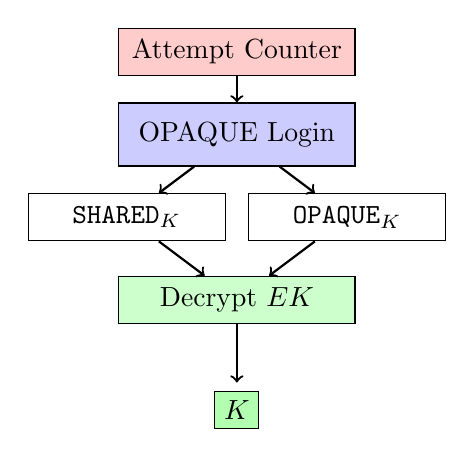
\begin{tikzpicture}[scale=0.7]
				% Attempt counter
				\node[draw, rectangle, minimum width=3cm, minimum height=0.6cm, fill=red!20] (counter) at (0,4) {Attempt Counter};

				% OPAQUE login
				\node[draw, rectangle, minimum width=3cm, minimum height=0.8cm, fill=blue!20] (opaque) at (0,2.5) {OPAQUE Login};
				\draw[->, thick] (counter) -- (opaque);

				% Keys derived
				\node[draw, rectangle, minimum width=2.5cm, minimum height=0.6cm] (shared) at (-2,1) {$\mathtt{SHARED}_K$};
				\node[draw, rectangle, minimum width=2.5cm, minimum height=0.6cm] (opaquek) at (2,1) {$\mathtt{OPAQUE}_K$};
				\draw[->, thick] (opaque) -- (shared);
				\draw[->, thick] (opaque) -- (opaquek);

				% Decryption
				\node[draw, rectangle, minimum width=3cm, minimum height=0.6cm, fill=green!20] (decrypt) at (0,-0.5) {Decrypt $EK$};
				\draw[->, thick] (shared) -- (decrypt);
				\draw[->, thick] (opaquek) -- (decrypt);

				% Result
				\node[draw, rectangle, fill=green!30] at (0,-2.5) {$K$};
				\draw[->, thick] (decrypt) -- (0,-2);
			\end{tikzpicture}
		\end{column}
	\end{columns}
\end{frame}

\begin{frame}{Security features}
	\begin{columns}[c]
		\begin{column}{0.5\textwidth}
			\textbf{Brute-force protection}
			\begin{itemize}
				\item HSM enforces attempt limits
				\item After threshold: Key permanently inaccessible
				\item Rate limiting in hardware
			\end{itemize}
		\end{column}
		\begin{column}{0.5\textwidth}
			\textbf{Infrastructure resilience}
			\begin{itemize}
				\item Deployed across seven or more data-center sites (2026 whitepaper)
				\item Majority-consensus replication
				\item Tolerates a failed replica and a disconnected site at once
			\end{itemize}
		\end{column}
	\end{columns}
	\vspace{0.5cm}
	\begin{center}
		\textbf{Transport security:} Noise Protocol Framework for client-server communication (here used as an alternative to TLS, but in reality it's a whole thing that lets you design a wide variety of protocols)
	\end{center}
\end{frame}

\begin{frame}{Alternative: user-managed 64-digit key}
	\begin{columns}[c]
		\begin{column}{1\textwidth}
			\begin{itemize}
				\item \textbf{For users who prefer full control:}
				      \begin{itemize}
					      \item 64-digit encryption key option
					      \item Key never sent to WhatsApp
					      \item User must store key securely
				      \end{itemize}
				\item \textbf{Trade-offs:}
				      \begin{itemize}
					      \item[\textcolor{green}{\mycheckmark}] Maximum security --- no trust required
					      \item[\textcolor{green}{\mycheckmark}] No brute-force risk
					      \item[\textcolor{red}{$\times$}] User responsibility for key management
					      \item[\textcolor{red}{$\times$}] Lost key = lost backups forever
				      \end{itemize}
				\item \textbf{Recommendation:} Only for technically sophisticated users
			\end{itemize}
		\end{column}
	\end{columns}
\end{frame}

\begin{frame}{What WhatsApp got right}
	\begin{itemize}
		\item \textbf{A standard protocol instead of a homebrew one:} OPAQUE, with a published security proof --- compare MEGA's AES-ECB key wrapping and custom RSA padding
		\item \textbf{A stated threat model:} the cloud provider, an outside attacker, and brute force on the password are in scope; WhatsApp's own HSMs are trusted
		\item \textbf{A published whitepaper}, later formally analyzed in the UC framework (Davies et al., CRYPTO 2023)\footnote{Gareth T. Davies, Sebastian Faller, Kai Gellert, Tobias Handirk, Julia Hesse, M\'at\'e Horv\'ath and Tibor Jager, \textit{Security Analysis of the WhatsApp End-to-End Encrypted Backup Protocol}, CRYPTO 2023.} --- under the assumption that the HSM is honest
		\item \textbf{User choice:} password + HSM vault, a self-managed 64-digit key, or (since 2025) a passkey
		\item \textbf{Complexity hidden:} the user sees a password prompt; the OPRF, the AKE and the HSM consensus are invisible
	\end{itemize}
	\vspace{0.3cm}
	\begin{center}
		\textit{Now let's look at what that threat model leaves out.}
	\end{center}
\end{frame}

\subsection{Critiquing WhatsApp's Design}

\begin{frame}{Specification ambiguity: a flaw in the whitepaper}
	\begin{itemize}
		\item \textbf{The problem:} the whitepaper calls $\mathtt{OPAQUE}_K$ ``a symmetric key which is used to secure the backup key $K$'' --- and never says \textit{which} OPAQUE output it is
		\item \textbf{Two candidates:}
		      \begin{itemize}
			      \item \textbf{Export key:} known to the client only
			      \item \textbf{Session key:} shared with the server
		      \end{itemize}
		\item \textbf{Why it matters:} if it were the session key, the vault could decrypt $K$ directly --- the whole point of the design would be gone
		\item \textbf{Resolving it takes outside knowledge:} the key is output by \textit{registration}, which in OPAQUE involves no key exchange, so it must be the export key; the login flow also lists $\mathtt{SHARED}_K$ separately
		\item \textbf{Lesson:} a cryptographic specification must be unambiguous \textit{on its own}. Two implementers reading this document could make different choices --- and one of them would be catastrophic
	\end{itemize}
\end{frame}

\begin{frame}{What you have to take on faith}
	\begin{columns}[c]
		\begin{column}{0.5\textwidth}
			\textbf{What WhatsApp claims:}
			\begin{itemize}
				\item Keys live in HSMs, and only there
				\item Attempt limits are enforced in hardware
				\item The vault runs the code described in the whitepaper
				\item No backdoor access, for anyone
			\end{itemize}
		\end{column}
		\begin{column}{0.5\textwidth}
			\textbf{What a user can check:}
			\begin{itemize}
				\item Since 2026: \textit{which public keys} the vault fleet uses, via a Cloudflare-run transparency log and Meta's open-source audit tool
				\item Everything else: nothing. No remote attestation, no independent audit, closed source
				\item ``Evidence of secure deployment'' is a Meta blog post
			\end{itemize}
		\end{column}
	\end{columns}
	\vspace{0.2cm}
	\begin{center}
		The HSMs are owned, operated and programmed by the very party the backups are meant to keep out.
	\end{center}
\end{frame}

\begin{frame}{Potential vulnerabilities in WhatsApp's design}
	\begin{columns}[c]
		\begin{column}{1\textwidth}
			\begin{itemize}
				\item \textbf{Silent key escrow:}
				      \begin{itemize}
					      \item HSM could have backdoor for data extraction
					      \item HSM could literally be one guy in a basement memorizing everything
					      \item No way for users to detect this
				      \end{itemize}
				\item \textbf{Selective targeting:}
				      \begin{itemize}
					      \item Different behavior for specific accounts
					      \item Disable rate limiting for law enforcement
					      \item Return fake ``attempt exceeded'' to user
				      \end{itemize}
				\item \textbf{Implementation substitution:}
				      \begin{itemize}
					      \item Replace HSM with software for some users
					      \item Use weaker entropy for key generation
					      \item Log passwords before OPAQUE processing
				      \end{itemize}
			\end{itemize}
		\end{column}
	\end{columns}
\end{frame}

\begin{frame}{The attestation problem}
	\begin{columns}[c]
		\begin{column}{0.5\textwidth}
			\begin{itemize}
				\item \textbf{What's missing:}
				      \begin{itemize}
					      \item Remote attestation from the HSMs
					      \item Cryptographic proof that the logged keys live in an HSM running the published code
					      \item Independent third-party verification
				      \end{itemize}
				\item \textbf{Technical solutions exist:}
				      \begin{itemize}
					      \item HSMs can provide attestation
					      \item Intel SGX, AMD SEV offer remote attestation
					      \item Transparency logs (\`a la Certificate Transparency)
				      \end{itemize}
			\end{itemize}
		\end{column}
		\begin{column}{0.5\textwidth}
			\begin{itemize}
				\item \textbf{Why not implemented?}
				      \begin{itemize}
					      \item Complexity for users?
					      \item Business reasons?
					      \item Legal requirements?
					      \item Law enforcement pressure?
				      \end{itemize}
				\item \textbf{The irony:} Meta runs key transparency for WhatsApp identity keys (2023) and, since 2026, for the vault's fleet keys --- but a transparency log proves \textit{which} keys are in use, not \textit{what} runs behind them
			\end{itemize}
		\end{column}
	\end{columns}
\end{frame}

\begin{frame}{Law enforcement pressure?}
	\begin{columns}[c]
		\begin{column}{0.5\textwidth}
			\imagewithcaption{cloud-pressure-a.png}{Source: Reuters}
		\end{column}
		\begin{column}{0.5\textwidth}
			\imagewithcaption{cloud-pressure-b.png}{Source: \url{https://support.apple.com/en-us/122234}}
		\end{column}
	\end{columns}
\end{frame}

\begin{frame}{The 64-digit key mystery}
	\begin{columns}[c]
		\begin{column}{0.5\textwidth}
			\begin{itemize}
				\item \textbf{What is the 64-digit key, really?}
				      \begin{itemize}
					      \item The whitepaper says only ``64-digit encryption key''; 64 decimal digits carry ${\approx}$212 bits, so it is not simply $K$ written out
					      \item No checksum or error detection mentioned
					      \item Hard to transcribe and store correctly
				      \end{itemize}
				\item \textbf{We already have friendlier encodings:}
				      \begin{itemize}
					      \item BIP39 mnemonics: 12--24 words with a checksum, proven by a decade of crypto wallets
				      \end{itemize}
			\end{itemize}
		\end{column}
		\begin{column}{0.5\textwidth}
			\begin{itemize}
				\item \textbf{Possible explanations:}
				      \begin{itemize}
					      \item Deliberate friction to push the HSM option?
					      \item Word lists are hard to localize across languages?
				      \end{itemize}
				\item \textbf{The industry hasn't settled this:}
				      \begin{itemize}
					      \item Signal's Secure Backups (2025) also use a 64-character recovery key
					      \item WhatsApp added passkey-encrypted backups (2025),\footnote{\url{https://about.fb.com/news/2025/10/making-it-easier-to-encrypt-whatsapp-chat-backups/}} hiding the key behind device biometrics
				      \end{itemize}
			\end{itemize}
		\end{column}
	\end{columns}
\end{frame}

\begin{frame}{A more honest assessment of WhatsApp backups}
	\begin{columns}[c]
		\begin{column}{1\textwidth}
			\begin{itemize}
				\item \textbf{What WhatsApp backups actually provide:}
				      \begin{itemize}
					      \item Protection from cloud providers (Google/Apple)
					      \item Some protection from external hackers
					      \item Convenient key recovery
				      \end{itemize}
				\item \textbf{What they DON'T provide:}
				      \begin{itemize}
					      \item Full protection from WhatsApp itself
					      \item Fully verifiable security guarantees
				      \end{itemize}
				\item \textbf{Alternatives:}
				      \begin{itemize}
					      \item Threshold cryptography across providers (Signal's SVR3)
					      \item Client-side key derivation only
					      \item Transparent, auditable systems
				      \end{itemize}
			\end{itemize}
		\end{column}
	\end{columns}
\end{frame}

\begin{frame}{Discussion time}
	\begin{columns}[c]
		\begin{column}{0.8\textwidth}
			\begin{enumerate}
				\item \textbf{Password + HSM vault, or a 64-digit key on paper?}
				      \begin{itemize}
					      \item Which would you pick for yourself? For your parents?
					      \item Does either pass the mud puddle test?
				      \end{itemize}
				\item \textbf{``Trust our hardware'' vs.\ ``trust our servers''}
				      \begin{itemize}
					      \item Is an HSM you cannot inspect meaningfully better than a plain server you cannot inspect?
					      \item What would it take to convince you? Remote attestation? Signal's three-vendor split? Open source?
				      \end{itemize}
				\item \textbf{Apple withdrew ADP from the UK rather than add a backdoor.} Was that the right call? What should WhatsApp do if it receives the same order?
			\end{enumerate}
		\end{column}
	\end{columns}
\end{frame}

\section{Designing an End-to-End Cloud Storage Protocol}

\subsection{Lessons Learned}

\begin{frame}{Security definitions matter}
	\begin{columns}[c]
		\begin{column}{1\textwidth}
			\textbf{MEGA's mistake:} Assumed encryption provides integrity
			\begin{itemize}
				\item Used AES-ECB without MAC
				\item Encryption $\neq$ Authenticated encryption
				\item Led to complete key recovery
			\end{itemize}
			\textbf{Nextcloud's mistake:} Assumed encryption provides authentication
			\begin{itemize}
				\item RSA-OAEP only provides confidentiality
				\item Anyone can create valid ciphertexts
				\item Led to key insertion attacks
			\end{itemize}
			\textbf{Sync, pCloud (2024):} same mistake as Nextcloud, made independently
			\vspace{0.2cm}

			\textbf{Lesson:} understand exactly what each primitive guarantees --- ``it encrypts, so it's secure'' is how every one of these systems was designed
		\end{column}
	\end{columns}
\end{frame}

\begin{frame}{What a sound design needs}
	\begin{enumerate}
		\item \textbf{A written threat model.} Malicious server, or merely curious? Writing down ``the server may modify what it stores'' would have flagged every MEGA attack
		\item \textbf{Standard primitives, used for what they guarantee.} AEAD wherever integrity matters (everywhere); no ECB, no bare RSA, no PKE where you need authentication
		\item \textbf{A key hierarchy that fits on one slide.} A random master key wrapped under a password-derived key, so passwords can change without re-encrypting everything
		\item \textbf{A proof, before deployment.} TLS 1.3 and Signal (topics 2.1, 2.3) were analyzed \textit{while} being designed; MEGA and Nextcloud by strangers, afterwards
	\end{enumerate}
	\vspace{0.2cm}
	\begin{center}
		\textit{The paper we look at next does all four.}
	\end{center}
\end{frame}

\begin{frame}{Reminder: formal analysis}
	\begin{columns}[c]
		\begin{column}{0.5\textwidth}
			\begin{itemize}
				\item \textbf{What is formal analysis?}\footnote{Coming up next, in topic 2.5: High-Assurance Cryptography!}
				      \begin{itemize}
					      \item Precise security definitions (our libraries from Part 1)
					      \item Proofs by reduction to hard problems
					      \item Increasingly: machine-checked, with software
				      \end{itemize}
				\item \textbf{Benefits:}
				      \begin{itemize}
					      \item Catches subtle flaws
					      \item Provides confidence
					      \item Clear security guarantees
					      \item Guides implementation
				      \end{itemize}
			\end{itemize}
		\end{column}
		\begin{column}{0.5\textwidth}
			\begin{itemize}
				\item \textbf{Types of analysis:}
				      \begin{itemize}
					      \item \textbf{Computational:} Reduction to hard problems
					      \item \textbf{Symbolic:} Protocol logic verification
					      \item \textbf{UC Framework:} Composable security
					      \item \textbf{Game-based:} Step-by-step proofs
				      \end{itemize}
				\item \textbf{Tools available:}
				      \begin{itemize}
					      \item ProVerif, Tamarin
					      \item EasyCrypt, CryptoVerif
					      \item \fstar
				      \end{itemize}
			\end{itemize}
		\end{column}
	\end{columns}
\end{frame}

\subsection{A Formal Treatment of End-to-End Encrypted Cloud Storage}

\begin{frame}{Next: a formal treatment from the literature}
	\begin{center}
		\textbf{What follows is based on:}\\
		\vspace{0.3cm}
		\textit{``A Formal Treatment of End-to-End Encrypted Cloud Storage''}\\
		{\tiny\url{https://appliedcryptography.page/paper/\#cloud-storage}}\\
		\vspace{0.2cm}
		{\footnotesize by Matilda Backendal, Hannah Davis, Felix G\"unther, Miro Haller, and Kenneth G. Paterson --- CRYPTO 2024}
	\end{center}
	\begin{columns}[t]
		\begin{column}{0.5\textwidth}
			\begin{itemize}
				\item \textbf{Why this paper?}
				      \begin{itemize}
					      \item First comprehensive formal treatment of E2EE cloud storage
					      \item Addresses the exact failures we've seen in MEGA/Nextcloud
					      \item Shows how to do protocol design \textit{right}
				      \end{itemize}
			\end{itemize}
		\end{column}
		\begin{column}{0.5\textwidth}
			\begin{itemize}
				\item \textbf{Key contributions:}
				      \begin{itemize}
					      \item Formal security definitions for E2EE storage
					      \item Clean, analyzable protocol design
					      \item Game-based security proofs
				      \end{itemize}
			\end{itemize}
		\end{column}
	\end{columns}
\end{frame}

\begin{frame}{A formal treatment: building blocks}
	\begin{columns}[c]
		\begin{column}{1\textwidth}
			\textbf{Core cryptographic primitives:}
			\begin{itemize}
				\item \textbf{PRF (Pseudorandom Function):} $F: \bits^{\kappa} \times \bits^{*} \to \bits^{\kappa}$
				\item \textbf{MAC (Message Authentication Code):} For integrity verification
				\item \textbf{AEAD (Authenticated Encryption):} AES-GCM or ChaCha20-Poly1305
				\item \textbf{2HashDH OPRF:} Password-based key derivation with the server's help --- no pre-computation, nothing for outsiders to attack offline
			\end{itemize}
			\vspace{0.3cm}
			\textbf{Key insight:} Use standard, proven primitives --- don't invent new ones!
		\end{column}
	\end{columns}
\end{frame}

\begin{frame}{The 2HashDH OPRF: motivation}
	\begin{columns}[c]
		\begin{column}{1\textwidth}
			\begin{itemize}
				\item \textbf{Problem:} How to derive keys from passwords without server learning them?
				\item \textbf{Challenge:} Server needs to help with computation, but shouldn't learn password
				\item \textbf{Solution:} an Oblivious Pseudorandom Function (OPRF) --- the same idea as in OPAQUE
				      \begin{itemize}
					      \item Client has secret input (account ID + password)
					      \item Server has key $k$
					      \item Together compute $F(k, \text{input})$ without server learning input
				      \end{itemize}
				\item \textbf{In our protocol:}
				      \begin{itemize}
					      \item Client generates OPRF key during registration
					      \item Sends the key to the server --- so the key is honestly random, not server-chosen
					      \item Later uses OPRF to derive keys from password
				      \end{itemize}
			\end{itemize}
		\end{column}
	\end{columns}
\end{frame}

\begin{frame}{The 2HashDH OPRF: how it works}
	\begin{columns}[c]
		\begin{column}{1\textwidth}
			\textbf{Setup:} Group $\mathbb{G}$ of prime order $q$, hash functions $H_1$ and $H_2$\footnote{$H_1$ hashes onto the group (``hash-to-curve''); $H_2$ should be slow and memory-hard, so that learning $k$ doesn't make password guessing cheap.}
			\begin{itemize}
				\item \textbf{Goal:} Client computes $H_2(x, H_1(x)^k)$ without revealing $x$ to server
				\item \textbf{Protocol steps:}
				      \begin{enumerate}
					      \item Client picks random blinding factor $r \twoheadleftarrow \mathbb{Z}_q$
					      \item Client sends blinded value: $\alpha = H_1(x)^r$ to server
						            {\footnotesize\begin{itemize}
								            \item Client hashes their secret input $x$ to get $H_1(x)$, raises it to the power of $r$, and sends this ``blinded'' result to the server --- the server cannot determine $x$ from this
							            \end{itemize}}
					      \item Server computes: $\beta = \alpha^k = H_1(x)^{rk}$ and returns it
					      \item Client unblinds: $\beta^{1/r} = H_1(x)^k$
					            {\footnotesize\begin{itemize}
							            \item The client removes the blinding by raising the server's response to the power of $1/r$ (the multiplicative inverse of $r$), which cancels out the $r$ in the exponent, leaving just $H_1(x)^k$
						            \end{itemize}}
					      \item Client outputs: $y = H_2(x, \beta^{1/r})$
				      \end{enumerate}
			\end{itemize}
		\end{column}
	\end{columns}
\end{frame}

\begin{frame}{The 2HashDH OPRF: what it buys us}
	\begin{itemize}
		\item \textbf{Obliviousness:} for random $r$, $\alpha = H_1(x)^r$ is a uniformly random group element --- the server learns nothing about $x$, at registration or at any login
		\item \textbf{Pseudorandomness:} without $k$, the output $y$ is unpredictable --- a network attacker, or anyone who steals the client's transcript, has nothing to guess against
		\item \textbf{No pre-computation:} $k$ acts as a secret salt that is never sent to the client
		\item \textbf{What it cannot do:} the party holding $k$ (here, the server) can still run a dictionary attack after the fact --- which is why the paper wants $H_1$ and $H_2$ slow and memory-hard, and why the client picks $k$
		\item Same primitive as in OPAQUE and in WhatsApp's vault --- there, $k$ lives inside the HSM
	\end{itemize}
\end{frame}

\begin{frame}{Scheme architecture: clean key hierarchy}
	\begin{columns}[c]
		\begin{column}{0.6\textwidth}
			\begin{itemize}
				\item \textbf{Password-derived keys:}
				      \begin{itemize}
					      \item Raw secret $rw$ from OPRF
					      \item Key encryption key $k_{kek}$
					      \item MAC key $k_{mac}$
				      \end{itemize}
				\item \textbf{Master key ($k_{mk}$):}
				      \begin{itemize}
					      \item Randomly generated
					      \item Encrypted with $k_{kek}$
					      \item Enables password changes!
				      \end{itemize}
				\item \textbf{File keys:}
				      \begin{itemize}
					      \item Unique per file
					      \item Encrypted with master key
					      \item Shared via headers
				      \end{itemize}
			\end{itemize}
		\end{column}
		\begin{column}{0.4\textwidth}
			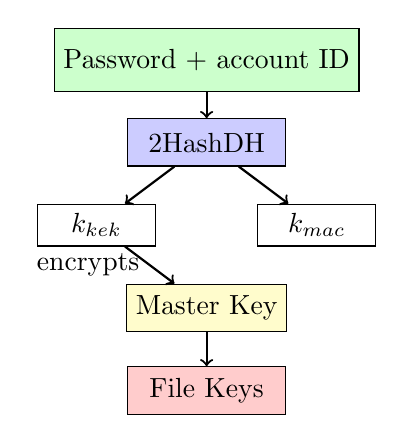
\begin{tikzpicture}[scale=0.7]
				% Password
				\node[draw, rectangle, minimum width=2.5cm, minimum height=0.8cm, fill=green!20] (password) at (0,5) {Password + account ID};

				% OPRF
				\node[draw, rectangle, minimum width=2cm, minimum height=0.6cm, fill=blue!20] (oprf) at (0,3.5) {2HashDH};
				\draw[->, thick] (password) -- (oprf);

				% Derived keys
				\node[draw, rectangle, minimum width=1.5cm, minimum height=0.5cm] (kkek) at (-2,2) {$k_{kek}$};
				\node[draw, rectangle, minimum width=1.5cm, minimum height=0.5cm] (kmac) at (2,2) {$k_{mac}$};
				\draw[->, thick] (oprf) -- (kkek);
				\draw[->, thick] (oprf) -- (kmac);

				% Master key
				\node[draw, rectangle, minimum width=2cm, minimum height=0.6cm, fill=yellow!20] (master) at (0,0.5) {Master Key};
				\draw[->, thick] (kkek) -- (master) node[midway, left] {encrypts};

				% File keys
				\node[draw, rectangle, minimum width=2cm, minimum height=0.6cm, fill=red!20] (filekeys) at (0,-1) {File Keys};
				\draw[->, thick] (master) -- (filekeys);
			\end{tikzpicture}
		\end{column}
	\end{columns}
\end{frame}

\begin{frame}{Registration and authentication flow}
	\begin{columns}[c]
		\begin{column}{0.5\textwidth}
			\textbf{Registration:}
			\begin{enumerate}
				\item Client samples OPRF key $k$, has account ID ($aid$)
				\item Computes $rw = \func{oprf}{aid, pw}$
				\item Derives $k_{kek}$, $k_{mac}$ from $rw$
				\item Generates random master key
				\item Encrypts master key with $k_{kek}$
				\item Sends to server: $aid$, $k$, $k_{mac}$, and the encrypted master key
			\end{enumerate}
		\end{column}
		\begin{column}{0.5\textwidth}
			\textbf{Authentication:}
			\begin{enumerate}
				\item Client initiates OPRF with server
				\item Server sends session ID ($sid$)
				\item Client recovers $rw$, derives keys
				\item Client MACs transcript with $k_{mac}$
				\item Server verifies MAC
				\item Server returns encrypted master key
				\item Client decrypts master key
			\end{enumerate}
		\end{column}
	\end{columns}
\end{frame}

\begin{frame}{File operations: simple and secure}
	\begin{columns}[c]
		\begin{column}{0.5\textwidth}
			\textbf{Upload (put):}
			\begin{itemize}
				\item Generate random file key
				\item AEAD-encrypt file with file key
				\item AEAD-encrypt file key with master key
				\item Store header (encrypted file key)
				\item Store encrypted file content
			\end{itemize}
		\end{column}
		\begin{column}{0.5\textwidth}
			\textbf{Download (get):}
			\begin{itemize}
				\item Fetch encrypted header
				\item Decrypt file key with master key
				\item Fetch encrypted file
				\item Decrypt file with file key
				\item All bound to file ID via AEAD
			\end{itemize}
		\end{column}
	\end{columns}
	\vspace{0.5cm}
	\begin{center}
		Separating headers from content enables efficient sharing!
	\end{center}
\end{frame}

\begin{frame}{Sharing design: each owner has their own header}
	\begin{columns}[c]
		\begin{column}{0.6\textwidth}
			\begin{itemize}
				\item \textbf{Sharing process:}
				      \begin{enumerate}
					      \item Owner fetches file key
					      \item Shares key out-of-band
					      \item Server adds new owner
					      \item Recipient wraps the key under their master key
				      \end{enumerate}
				\item \textbf{Benefits:}
				      \begin{itemize}
					      \item No re-encryption on updates
					      \item Independent key management
					      \item Efficient for large files
					      \item Password changes don't affect shares
				      \end{itemize}
			\end{itemize}
		\end{column}
		\begin{column}{0.4\textwidth}
			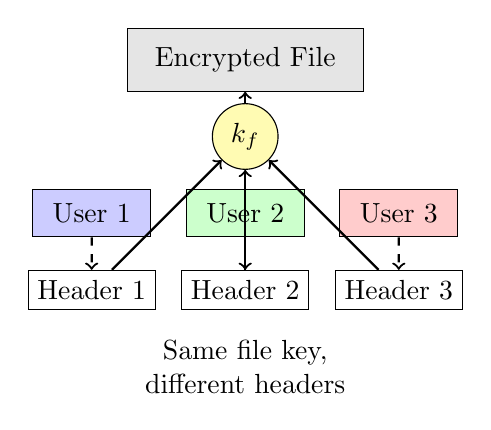
\begin{tikzpicture}[scale=0.65]
				% File
				\node[draw, rectangle, minimum width=3cm, minimum height=0.8cm, fill=gray!20] (file) at (0,3) {Encrypted File};

				% File key
				\node[draw, circle, fill=yellow!30] (filekey) at (0,1.5) {$k_f$};

				% Users
				\node[draw, rectangle, minimum width=1.5cm, minimum height=0.6cm, fill=blue!20] (user1) at (-3,0) {User 1};
				\node[draw, rectangle, minimum width=1.5cm, minimum height=0.6cm, fill=green!20] (user2) at (0,0) {User 2};
				\node[draw, rectangle, minimum width=1.5cm, minimum height=0.6cm, fill=red!20] (user3) at (3,0) {User 3};

				% Headers
				\node[draw, rectangle, minimum width=1.2cm, minimum height=0.5cm] (h1) at (-3,-1.5) {Header 1};
				\node[draw, rectangle, minimum width=1.2cm, minimum height=0.5cm] (h2) at (0,-1.5) {Header 2};
				\node[draw, rectangle, minimum width=1.2cm, minimum height=0.5cm] (h3) at (3,-1.5) {Header 3};

				% Connections
				\draw[->, thick] (filekey) -- (file);
				\draw[->, thick, dashed] (user1) -- (h1);
				\draw[->, thick, dashed] (user2) -- (h2);
				\draw[->, thick, dashed] (user3) -- (h3);
				\draw[->, thick] (h1) -- (filekey);
				\draw[->, thick] (h2) -- (filekey);
				\draw[->, thick] (h3) -- (filekey);

				\node[text width=3cm, align=center] at (0,-3) {Same file key, different headers};
			\end{tikzpicture}
		\end{column}
	\end{columns}
\end{frame}

\begin{frame}{Security properties achieved}
	\begin{columns}[c]
		\begin{column}{0.5\textwidth}
			\textbf{Against malicious server:}
			\begin{itemize}
				\item[\textcolor{green}{\mycheckmark}] No pre-computation, nothing for outsiders to attack offline (OPRF)
				\item[\textcolor{green}{\mycheckmark}] Authenticated encryption throughout
				\item[\textcolor{green}{\mycheckmark}] Account ID in the OPRF input: users sharing a password get unrelated keys, so the server can't swap their files
			\end{itemize}
		\end{column}
		\begin{column}{0.5\textwidth}
			\textbf{Design advantages:}
			\begin{itemize}
				\item[\textcolor{green}{\mycheckmark}] Password changes without re-encryption
				\item[\textcolor{green}{\mycheckmark}] Efficient file sharing
				\item[\textcolor{green}{\mycheckmark}] Simple, analyzable design
				\item[\textcolor{green}{\mycheckmark}] Uses only standard primitives
			\end{itemize}
		\end{column}
	\end{columns}
	\vspace{0.5cm}
	\begin{center}
		\textbf{This scheme has formal security proofs!}
	\end{center}
\end{frame}

\begin{frame}{Comparing with MEGA/Nextcloud}
	\begin{columns}[c]
		\begin{column}{0.33\textwidth}
			\textbf{MEGA}
			\begin{itemize}
				\item[\textcolor{red}{$\times$}] Custom crypto
				\item[\textcolor{red}{$\times$}] No AEAD
				\item[\textcolor{red}{$\times$}] Complex design
				\item[\textcolor{red}{$\times$}] No formal analysis
			\end{itemize}
		\end{column}
		\begin{column}{0.33\textwidth}
			\textbf{Nextcloud}
			\begin{itemize}
				\item[\textcolor{red}{$\times$}] Missing authentication
				\item[\textcolor{red}{$\times$}] Implementation bugs
				\item[\textcolor{red}{$\times$}] Ad-hoc design
				\item[\textcolor{red}{$\times$}] Nonce reuse
			\end{itemize}
		\end{column}
		\begin{column}{0.34\textwidth}
			\textbf{This scheme}
			\begin{itemize}
				\item[\textcolor{green}{\mycheckmark}] Standard primitives
				\item[\textcolor{green}{\mycheckmark}] AEAD everywhere
				\item[\textcolor{green}{\mycheckmark}] Clean hierarchy
				\item[\textcolor{green}{\mycheckmark}] Formal proofs
			\end{itemize}
		\end{column}
	\end{columns}
	\vspace{0.5cm}
	\begin{center}
		\textit{Simplicity and formal analysis make the difference!}
	\end{center}
\end{frame}

\begin{frame}{Key takeaways}
	\begin{columns}[c]
		\begin{column}{0.5\textwidth}
			\begin{itemize}
				\item \textbf{End-to-end encryption is hard to get right}
				      \begin{itemize}
					      \item Even major companies make critical mistakes
					      \item Ad-hoc designs inevitably fail
					      \item Retrofitting security doesn't work
				      \end{itemize}
				\item \textbf{Use established cryptographic building blocks}
				      \begin{itemize}
					      \item Don't roll your own crypto
					      \item Understand what primitives actually guarantee
					      \item Simplicity beats cleverness
				      \end{itemize}
			\end{itemize}
		\end{column}
		\begin{column}{0.5\textwidth}
			\begin{itemize}
				\item \textbf{Formal analysis is essential}
				      \begin{itemize}
					      \item Catches subtle vulnerabilities
					      \item Provides clear security guarantees
					      \item Should be done \textit{before} deployment
				      \end{itemize}
				\item \textbf{Trust models matter}
				      \begin{itemize}
					      \item Be honest about what you're protecting against
					      \item Users need verifiable security, not promises
					      \item Transparency builds trust
				      \end{itemize}
			\end{itemize}
		\end{column}
	\end{columns}
\end{frame}

\begin{frame}{\textit{And remember\ldots}}
	\begin{columns}[c]
		\begin{column}{0.5\textwidth}
			\begin{center}
				{\Large The best cryptographic protocol is one that's\\
					\textit{simple enough to understand} and \textit{proven to be secure}} \\
				\vspace{1cm}
				{\small\textit{``Complexity is the enemy of security''}}
			\end{center}
		\end{column}
		\begin{column}{0.5\textwidth}
			\imagewithcaption{spamton-sez.png}{}
		\end{column}
	\end{columns}
\end{frame}

\begin{frame}[plain]
	\titlepage
\end{frame}
\end{document}
